\documentclass[fleqn,10pt]{wlscirep}
\usepackage[utf8]{inputenc}
\usepackage[T1]{fontenc}
\usepackage{bm}
\usepackage{caption}
\usepackage{subcaption}
% \captionsetup[subfigure]{justification=justified,singlelinecheck=false}
\usepackage{tikz}
\usepackage{newtxmath} % MER: Prettier math
\usepackage{cleveref} % MER: Allows \Cref (but use Section X.Y not Subsection X.Y)
\usepackage{booktabs} % MER: Prettier tables

\usepackage{graphicx}
\usepackage{subcaption}
\usepackage{tikz}
\usepackage{float}
\usepackage{amsmath}
\usepackage{siunitx}
\usetikzlibrary{quotes}
\usetikzlibrary{arrows,decorations.pathmorphing,backgrounds,positioning,fit,petri}

\graphicspath{{figures/}}

\captionsetup[subfigure]{justification=justified,singlelinecheck=false}

\title{In-silico molecular transport in the human intracranial space}

\author[1,x]{Rami Masri}
\author[1,x]{Miroslav Kuchta}
\author[1,x]{Marius Causemann}
\author[1,*]{Marie E. Rognes}
\affil[1]{Department of Numerical Analysis and Scientific Computing, Simula Research Laboratory, Oslo, Norway}
\affil[x]{Author order to be discussed.}
\affil[*]{meg@simula.no}

\newcommand{\rami}[1]{\textcolor{blue}{#1}}
\newcommand{\mer}[1]{\textcolor{magenta}{#1}}
\newcommand{\mar}[1]{\textcolor{violet}{#1}}
\newcommand{\discuss}[1]{\textcolor{red}{#1}}
\newcommand{\draft}[1]{\textcolor{gray}{#1}}
\newcommand{\brain}{\Omega_{\rm{PAR}}} 
\newcommand{\sas}{\Omega_{\rm CSF}}
\newcommand{\pia}{\Gamma_{\rm{Pia}}}
\newcommand{\spinal}{\Gamma_{\rm SAS}}
\newcommand{\skull}{\Gamma_{\rm{skull}}}
\newcommand{\gin}{g_{\rm{influx}}}
 % Hello darkness my old friend. I've come to talk with you again. 

%\affil[+]{these authors contributed equally to this work}

%\keywords{Keyword1, Keyword2, Keyword3}

\begin{abstract}
\end{abstract}
\begin{document}

\flushbottom
\maketitle
% * <john.hammersley@gmail.com> 2015-02-09T12:07:31.197Z:
%
%  Click the title above to edit the author information and abstract
%
\thispagestyle{empty}


%%%%%%%%%%%%%%%%%%%%%%%%%%%%%%%%%%%%%%%%%%%%%%%%%%%%%%%%%%%%%%%%%%%%%%%%%%%%%%%%%%%%%

\mer{MER: Target length: 5000 words, 4-6 figures.}

\section*{Introduction}


Molecular transport in perivascular spaces (PVSs) is established as a key pathway for human brain clearance and delivery. Previous studies indicate that molecules move rapidly in the subarachnoid space (SAS) and in PVSs surrounding pial arteries. Here, we aim to model and study this transport in a full pial perivascular and/or vascular network embedded in the SAS.  

Motivation: as indicated by~\cite{iliff2012paravascular}, referring to
Cserr, Phys Rev., 1971, bulk convective flow may be more important for
larger species (larger distances) and larger molecules.

\section*{Background}

\mer{Point from Miro: Goriely and scaling from mice to men.}

\begin{enumerate}
\item
  Communication between perivascular spaces and the subarachnoid space
  \begin{itemize}
  \item
    Rennels et al~\cite{rennels1985evidence} infused tracer into the lateral cerebral ventricles and subarachnoid space of cats (and one dog) and observed that the tracer distributed in a perivascular pattern. The tracer distributed more rapidly around arterioles than around capillaries and veins. Importantly, the rapid paravascular influx was modulated by arterial pulsatility and in particular reduced by reduced vessel pulsatility. They directly postulate that ``fluid circulation through the central nervous system occurs via paravascular pathways'', and discuss both mixing and pumping as pulsatility-associated mechanisms for transport. 
  \item
    Weller and coauthors conducted pioneering studies of perivascular spaces, flow and transport~\cite{zhang1990interrelationships, zhang1992directional, weller2005microscopic}. They identified thin sheaths of pial cells surrounding arteries and arterioles (but not veins or venules) on the brain surface and within the human brain itself~\cite{zhang1990interrelationships}. Further, they observed that tracers spread along perivascular (arterial, venous and capillar) spaces in (rat) grey matter, and in the subarachnoid space (to the cribriform plate and nasal lymphatics).   
  \item
    Ichimura et al~\cite{ichimura1991distribution} study the distribution of large molecular weight tracers in the subarachnoid and surface perivascular spaces and within the cortex in rats. They observed rapid spread in perivascular spaces, and that tracers injected into the CSF of the subarachnoid space spread also into subarachnoid and cortical perivascular spaces. In conclusion, they highlight the presence of an extensive perivascular network, and report of some bulk flow, but slow and of variable directionality - in contrast to e.g Rennels et al~\cite{rennels1985evidence}. 
  \item In a series of papers, Bakker and coauthors study perivascular anatomy and solute transport~\cite{bedussi2017paravascular, bedussi2018paravascular}. They find that the subarachnoid space, the cisterns, ventricles and penetrating periarteriolar spaces form a continuous cerebrospinal fluid-filled space surrounding and penetrating into the murine brain \cite{bedussi2017paravascular}. Moreover, they demonstrate pulsatile and directional (antegrade) flow in perivascular (predominantly periarterial) spaces on the brain surface \cite{bedussi2018paravascular}. 
  \item
    Iliff et al~\cite{iliff2012paravascular} observed rapid movement of tracer (injected in the cisterna magna) along the outside of surface arteries and penetrating arterioles in mice, and state this is in agreement with the presence of perivascular sheaths as reviewed by Weller~\cite{weller2005microscopic}.
  \item
    The architecture of perivascular spaces in and around the rat brain was also studied in detail by Thorne and colleagues~\cite{pizzo2018intrathecal, hannocks2018molecular}. Hannocks et al~\cite{hannocks2018molecular} characterize the molecular composition of different perivascular compartments. Pizzo et al~\cite{pizzo2018intrathecal} emphasizes the presence of stomata or pores present on the interface between blood vessels and the CSF in the subarachnoid space. Neither seem to quantitatively report on PVS widths.
  \item Mestre et al~\cite{mestre2022periarteriolar} study the properties of pial perivascular spaces in detail in mice, and in particular the structure and coverage of pial cells and pial layers surrounding leptomeningeal arteries (and arterioles). They report of pial cells forming sheaths for larger ($> 10000 \mu$m$^2$ cross-section lumen area) surface arteries and partially coverage for smaller surface arteries, with higher coverage in ventral SAS regions. They find that these pial layers do not form an impermeable barrier to small molecules. Importantly, they also study the pial coverage in aged and Alzheimer's model mice, and find significant and complex changes in these pial structures.
  \item
    In humans, Eide and Ringstad investigate cerebrospinal fluid tracer transport in the human subarachnoid space after intrathecal injection~\cite{eide2024functional}. They observe tracer enrichment antegrade along the major cerebral arteries, and enrichment of the nearly cerebral cortex. They also consider variations in different patient cohorts and find impaired transport in iNPH patients with increased perivascular space size. They report of tracer enrichment in donut-shaped perivascular spaces. 
  \end{itemize}
\item
  Shapes and sizes of the perivascular spaces\footnote{The area $A$ of
  a circle with inner radius $R_1$ is $A = \pi R_1^2$. The area $A_2$
  of an annulus with inner radius $R_1$ and outer radius $R_2$ is $A_2
  = \pi (R_2^2 - R_1^2)$. The width of this annulus is $R_2 -
  R_1$. The ratio PVS/lumen area can thus be estimated as $A_2/A =
  (R_2^2 - R_1^2)/R_1^2$. For example, if $R_2 = n R_1$ ($n = 2
  \rightarrow$ PVS width equal to lumen radius, $n = 3 \rightarrow$
  PVS width equal to lumen diameter), then $A_2/A = n^2 - 1$. However,
  if the annulus has an elliptic outer boundary with radii $R_a$ and
  $R_b$, then its area is $A_e = \pi (R_a R_b - R_1^2)$, and so in the
  extreme case where $R_a > R_b = R_1$, the area is $\pi R_1 (R_a -
  R_1)$, and the PVS/lumen area ratio is $A_e/A = (R_a -
  R_1)/R_1$. And so, for $R_a = n R_1$, then $A_e/A = n-1$.}. Note
  that representing the surface PVS as annular cylinders is a
  simplification, and several studies emphasize the asymmetric nature
  of the PVS shape~\cite{mestre2018flow, tithof2019hydraulic,
    vinje2021brain, raicevic2023sizes}. Moreover, do not forget that
  the sizes of mice and humans are orders of magnitude apart.
  \begin{itemize}
  \item
    Ichimura et al~\cite{ichimura1991distribution} report on a typical
    perivascular width of $1-10\mu$m, but broader around vessel
    bifurcations in the rat subarachnoid space (fixed specimens).
  \item Foley et al~\cite{foley2012realtime} report on perivascular
    space width within rat cortex of $8-10\mu$m for arterioles of
    $\approx$30$\mu$m in diameter.
  \item
    Schain et al~\cite{schain2017cortical} report on the sizes of pial
    arteries ($6.0-11 \mu$m in diameter\footnote{Schain et
    al~\cite{schain2017cortical} state diameter rather, but the
    diameter does not match with the given area, so perhaps this
    should be the radius}) and veins ($9.4-21\mu$m) in mice, with an
    average PVS/lumen area ratio of $1.26$ for arteries and $0.13$ for
    veins. 
  \item Mestre et al~\cite{mestre2018flow} measure and characterize
    pial perivascular transport and estimate flow magnitudes in
    mice. They report a PVS/lumen area ratio of $1.4 \pm 0.1$ and a
    PVS width of $\approx 40 \mu$m which described as comparable to
    the adjacent artery (diameter). 
\item
  Raicevic et al~\cite{raicevic2023sizes} study the sizes and shapes
  of perivascular spaces surrounding pial arteries in mice in detail,
  in particular the relationship between periarterial space and lumen
  (cross-section) area and its variation with vessel area and
  location. They remark that the variation in PVS area is larger
  between PVS segments than along a single PVS segment. The PVS area
  seems to increase with the vessel area, but an affine approximation
  gives a poor fit, and from inspecting the distribution, the
  relationship seems superlinear. The peak distribution value of
  segmented PVS/lumen area is $1.12$.
  \item
    In terms of size, Bedussi et al.~\cite{bedussi2018paravascular} report a PVS width of $\approx$20$\mu$m surrounding surface arteries branching from the MCA (of diameters $45 \pm 7$ $\mu$m). 
  \item Vinje et al~\cite{vinje2021brain} and references therein illustrates the location and characteristics of human pial perivascular spaces, using human OCT data from the Bakker lab.
  \item Bollman et al~\cite{bollmann2022imaging} image the human pial vasculature at high resolution (7T), and report of pial arterial diameters in the range $50-280 \mu$m.
\item
  Smets et al~\cite{smets2024perivascular} study the size of
  perivascular spaces surrounding pial arteries and veins in mice
  (in-vivo), with particular emphasis on the properties of perivenous
  spaces. They observe the PVS as two ``triangular spaces'' adjacent
  to both arteries and veins, and separated from the subarachnoid
  space by a membrane (see also references
  to~\cite{zhang1990interrelationships, pizzo2018intrathecal,
    mollgard2023mesothelium}). They found that the cross-section area
  of the PVS correlates with the lumen area both for pial arteries
  and veins, but not for penetrating vessels. They report a
  PVS-to-lumen-area ratio of 0.43 for arteries and 0.35 for veins.
\item
  Personal communication (Ringstad, Oct 15 2024)~\cite{eide2024functional}: a typical blood vessel in the M2-segment of the MCA is 1.56 mm in diameter ($2 R_1$) with an annular PVS of width ($R_2 - R_1$) 1.23 mm and total PVS diameter $2 R_2$ of 3.93. In iNPH patients, extreme outliers are observed; e.g. still with annular PVS, but not concentric (shifted vessel), for vessel diameter of 2 mm and PVS width from 1.1 mm to 6.0 mm.
  \end{itemize}
\item
  Perivascular hydraulic resistances. The hydraulic resistance of
  perivascular spaces has been studied extensively, with key
  contributions from Thomas, Kelley, Tithof and collaborators~\cite{tithof2019hydraulic}.
  \begin{itemize}
  \item Boster et al.~\cite{boster2024hydraulic} study methods of estimating the hydraulic resistance of perivascular spaces via in-vivo imaging-based 3D reconstructions of pial perivascular spaces in mice; they report of hydraulic resistances of the order $1.7 \times 10^6 - 8.9 \times 10^5$ mmHg·min/mL/m).
  \end{itemize}
\item
  Perivascular flow characteristics: magnitudes and directionality?
  \begin{itemize}
  \item
    Rennels et al~\cite{rennels1985evidence} highlight in their
    Discussion that
    \begin{quote}
      This evidence of fluid displacement in both directions through
      the perivascular spaces suggest either that influx and efflux
      occur intermittently through the same perivascular spaces or
      that these fluid movements occur via separate populations of
      perivascular spaces.
    \end{quote}
  \item
    Ichimura et al~\cite{ichimura1991distribution} found that albumin in the subarachnoid periarterial space moved 1.5 mm away from the injection site in about 7 minutes, thus a net speed of around $3.6 \mu$m/s. 
  \item
    Hadaczek et al~\cite{hadaczek2006perivascular} studied the role of arterial pulsations in more detail, following up on~\cite{rennels1985evidence}.
  \item Foley et al~\cite{foley2012realtime} study perivascular transport characteristics of nanoparticles injected in the cerebral cortex of rats, though in the context of convection-enhanced delivery.
  \item
    In terms of movement, Bedussi et al~\cite{bedussi2018paravascular} found a net movement of particles in surface PVS (in mice) in the antegrade (same direction as blood flow) direction with an average velocity of $17 \pm 2\mu$m/s, and a mean amplitude of the pulsatile motion of $14 \pm 2 \mu$m.
\item Mestre et al~\cite{mestre2018flow} report a mean (averaged over time and space) flow speed of $18.7 \mu$m/s (root-mean-square velocity?) with net transport in the antegrade direction (near the MCA, in mice).
\item
  Asgari et al~\cite{asgari2016glymphatic} model tracer transport in axial periarterial spaces, highlight the negligible net (directional, bulk) flow induced by arterial wall pulsations at physiologically realistic wavelengths, but also the contributions from wall pulsations to dispersion. 
\item
  Rey and Sartinoranont~\cite{rey2018pulsatile} examine pulsatility as a driver for net flow in perivascular spaces within the brain parenchyma via a hydraulic network models, again highlighting the negligible net flow induced by vascular wall movements, but significant pulsatile flow and thus potential for dispersive effects~\cite{watson1983diffusion, asgari2016glymphatic}.
\item
  Rey et al~\cite{rey2023perivascular} consider a comprehensive ex-vivo perivascular network segmentation in the rat brain following in-vivo intraventricular contrast infusion. They highlight the numerous connections between the ventricular system and the perivascular spaces, including long perivascular segments extending from the surface and deep into the brain. 
\item
  In the context of dispersion, see also~\cite{asgari2016glymphatic, keith2019dispersion, troyetsky2021dispersion}
\item
  Wright et al~\cite{wright2024coupled} study the dynamics (waveforms over time) of human arterial blood flow (with resting-state fMRI) and perivascular CSF flow (with dynDWI, apparent diffusion coefficient (mm$^2$/s)). The waveforms seem coupled, with the arterial peak preceding the CSF peak by around 0.06 (of a cardiac cycle). The report ADC in the PVS on the order $2.5-5.5 \times 10^{-3}$ mm$^2$/s, with alterations in the coupling with age.
\item
  Boster and coauthors~\cite{boster2023artificial, toscano2024infeering} estimate perivascular flow parameters in mice via physics-informed neural networks (e.g.~pressure gradients, hydraulic resistances, shear stresses). Boster et al~\cite{boster2023artificial} estimate PVS pressure gradients on the order of $0.7-5 \times 10^{-4} \unit{Pa/\mu m}$\footnote{Note that 
  \begin{equation}
    1 \times 10^{-4} \, \unit{Pa/\mu m} = 1 \times 10^{2} \, \unit{Pa/m} \approx 100/133 \unit{mmHg/m} \approx 0.75 \unit{mmHg/m}
  \end{equation}
   }, downstream velocity component of $12.75 \pm 6.25 \unit{\mu m/s}$. 
  \end{itemize}
\end{enumerate}
Cerebrospinal fluid flow
\begin{itemize}
\item
  Vinje et al.~\cite{vinje2019respiratory} consider clinical measurements of intracranial pressure differences and human CSF-space geometries together with computational modelling to study CSF flow patterns in the aqueduct. They estimate the pressure gradient across the cerebral aqueduct resulting from a CSF production of 0.5L/day to be $0.009 \pm 0.006$ mmHg/m.
\item Hornkjøl et al~\cite{hornkjol2022csf} model CSF flow and solute transport in the human SAS and brain parenchyma. 
\end{itemize}

%%%%%%%%%%%%%%%%%%%%%%%%%%%%%%%%%%%%%%%%%%%%%%%%%%%%%%%%%%%%%%%%%%%%%%%%%%%%%%%%%%%%%
\section*{Results}

\subsection*{High-fidelity in-silico predictions of intracranial solute transport and exchange}

\begin{itemize}
\item
  Present mathematical and computational model and geometries (\Cref{tab:scenarios}). 
\item
  Highlight computational model availability, open source code.
\item
  Provides an interactive in-silico platform for studying intracranial solute transport -- distribute such that anyone can run (possibly try to recruit MinRK if advantageous).
\end{itemize}

\draft{\lipsum[1]}

\subsection*{II: CSF flow}

\mer{MER: @Marius: 2-3 sentences motivating the choice of production-induced flow and dispersion enhanced by pulsatility~\cite{ray2021quantitative}. 2-3 sentences summarizing what you computed. 4-6 sentences describing the flow and dispersion results.} \draft{\lipsum[1]} \Cref{fig:csf}
\begin{figure}[h!]
\centering 
\begin{subfigure}[b]{0.33\textwidth}
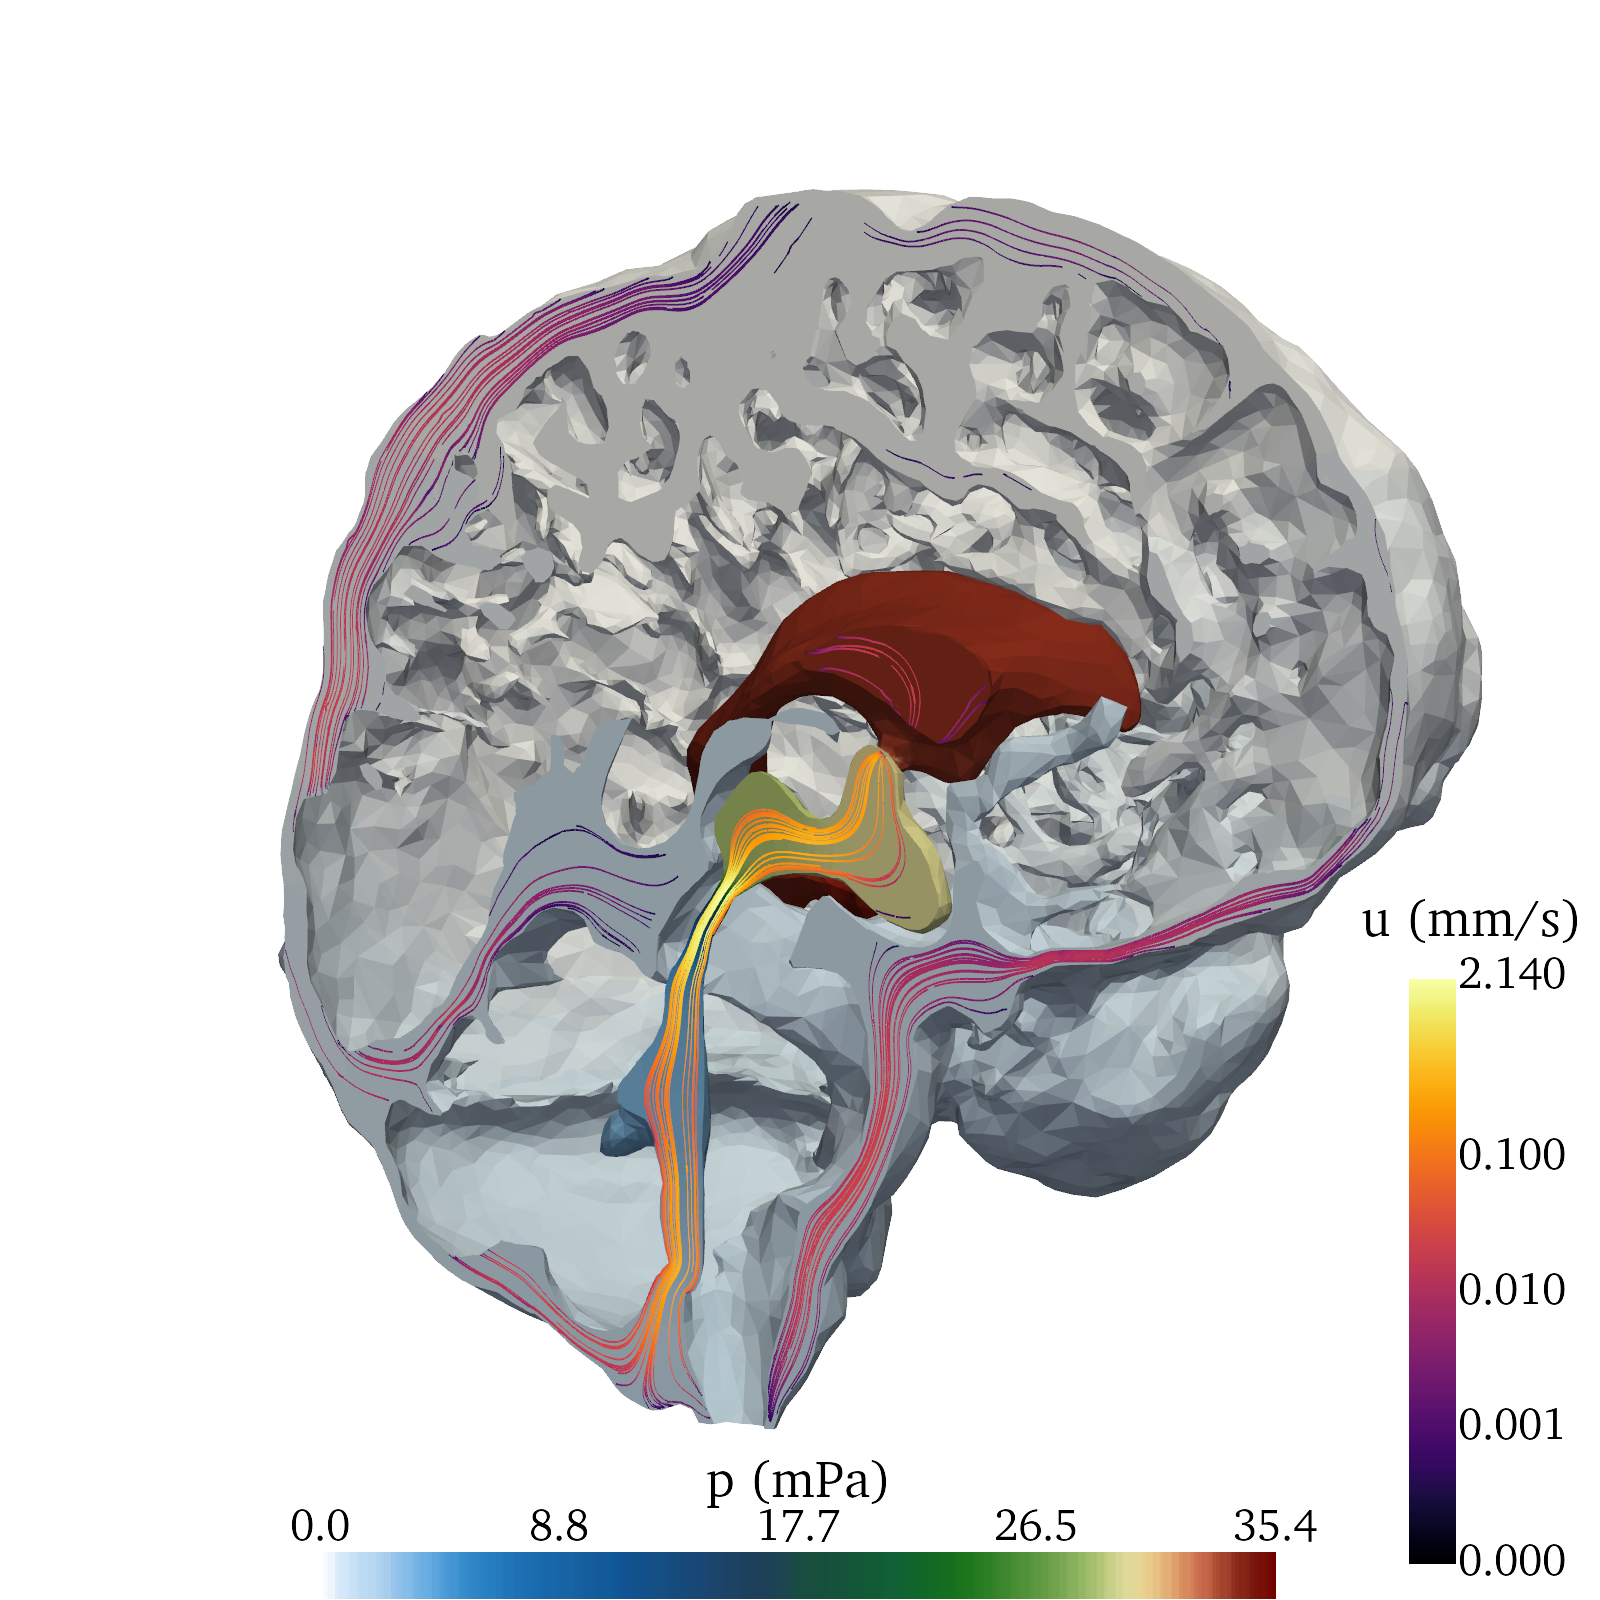
\includegraphics[width = 1 \textwidth]{figures/csf_v.png}
\caption{CSF flow from CSF production}
\label{fig:csf_flow_prod}
\end{subfigure}
\begin{subfigure}[b]{0.33\textwidth}
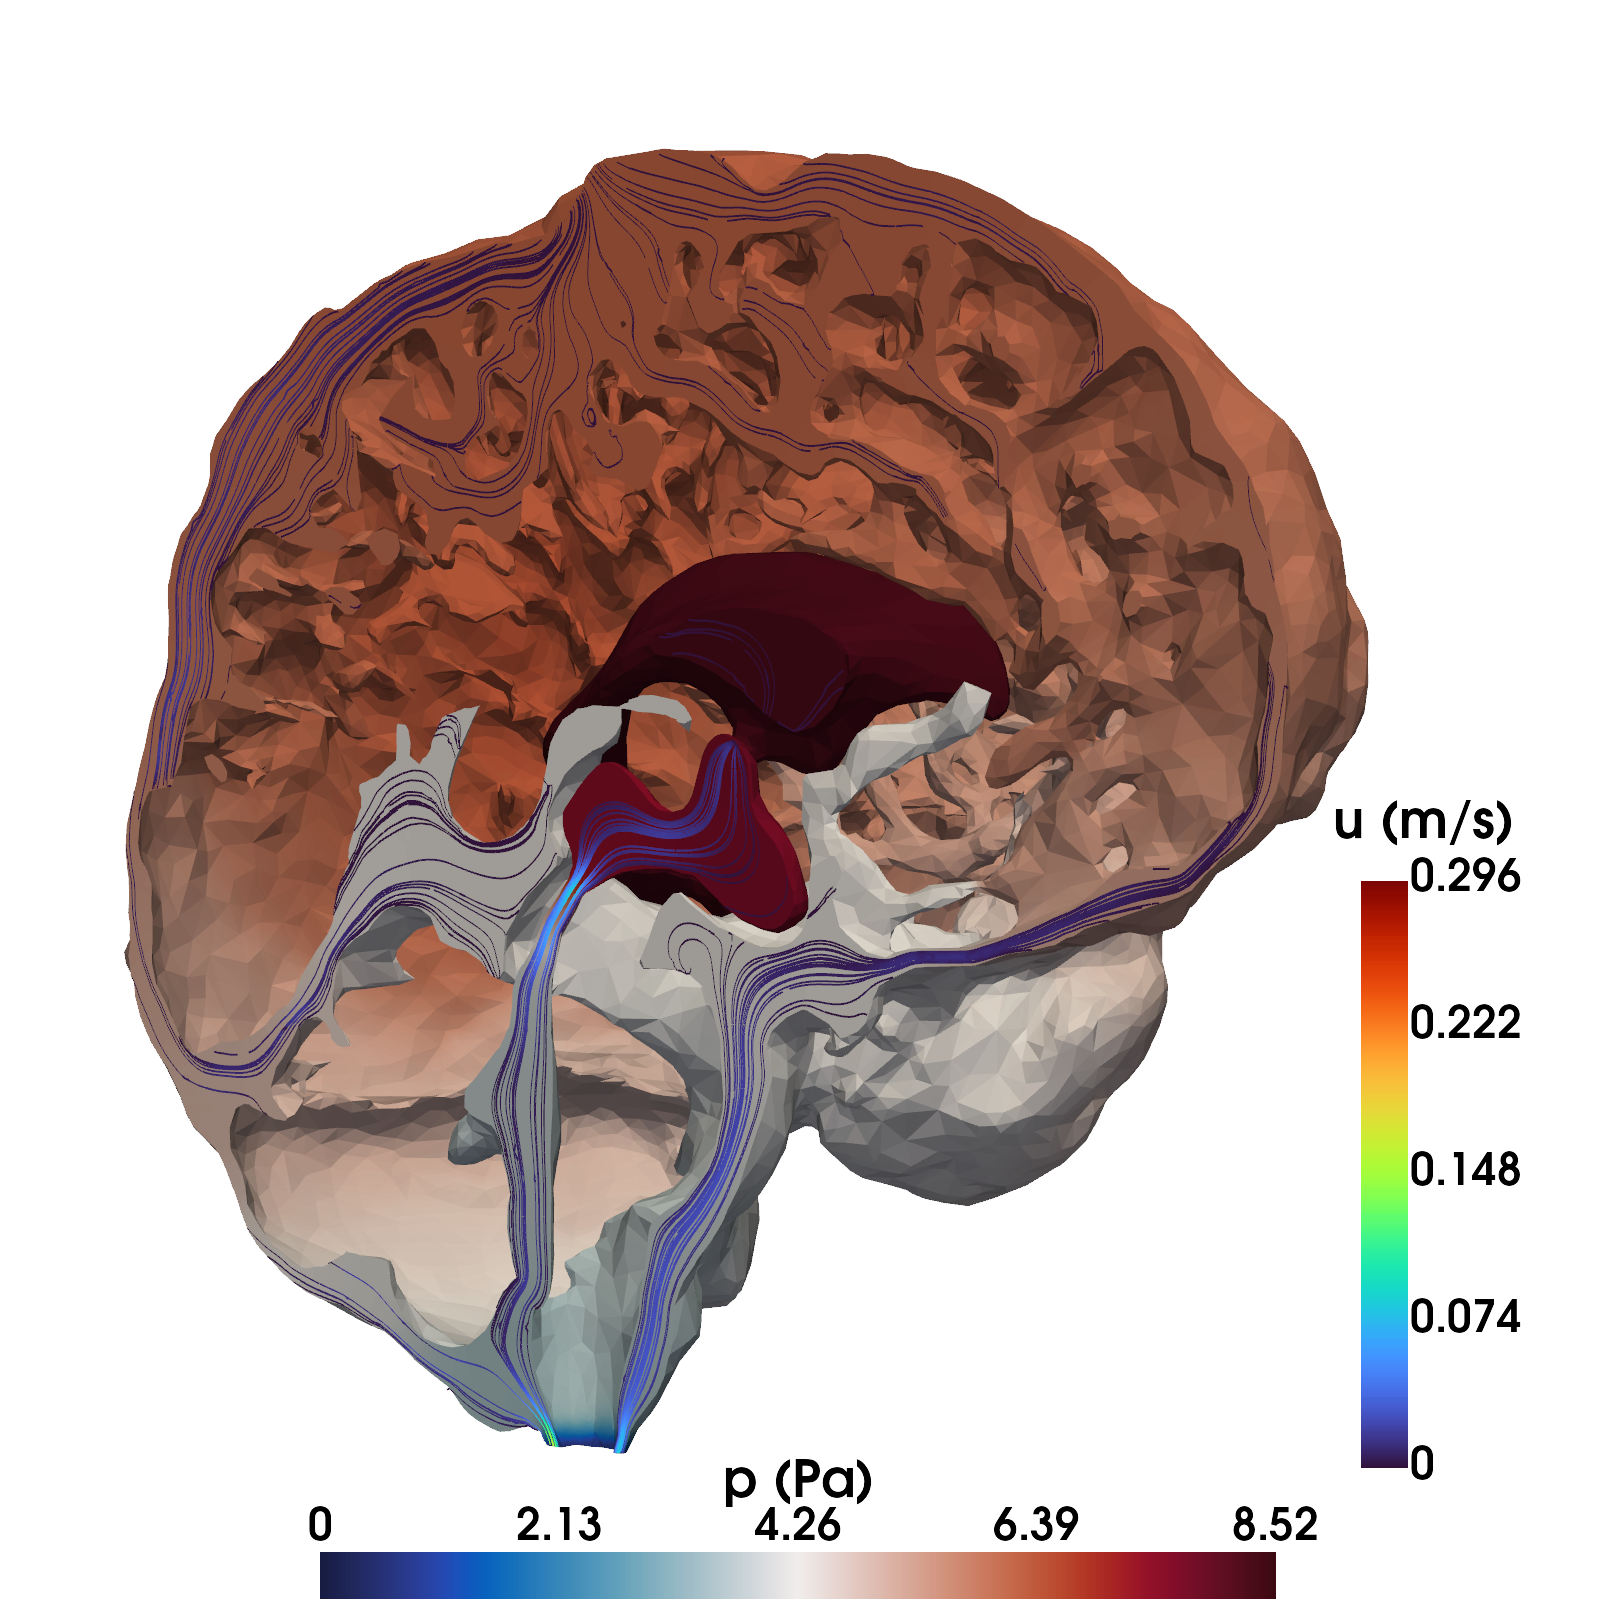
\includegraphics[width = 1 \textwidth]{figures/cardiac_csf_v.png}
\caption{CSF flow  from cardiac pulsatility}
\label{fig:csf_flow_cardiac}
\end{subfigure}
\begin{subfigure}[b]{0.33\textwidth}
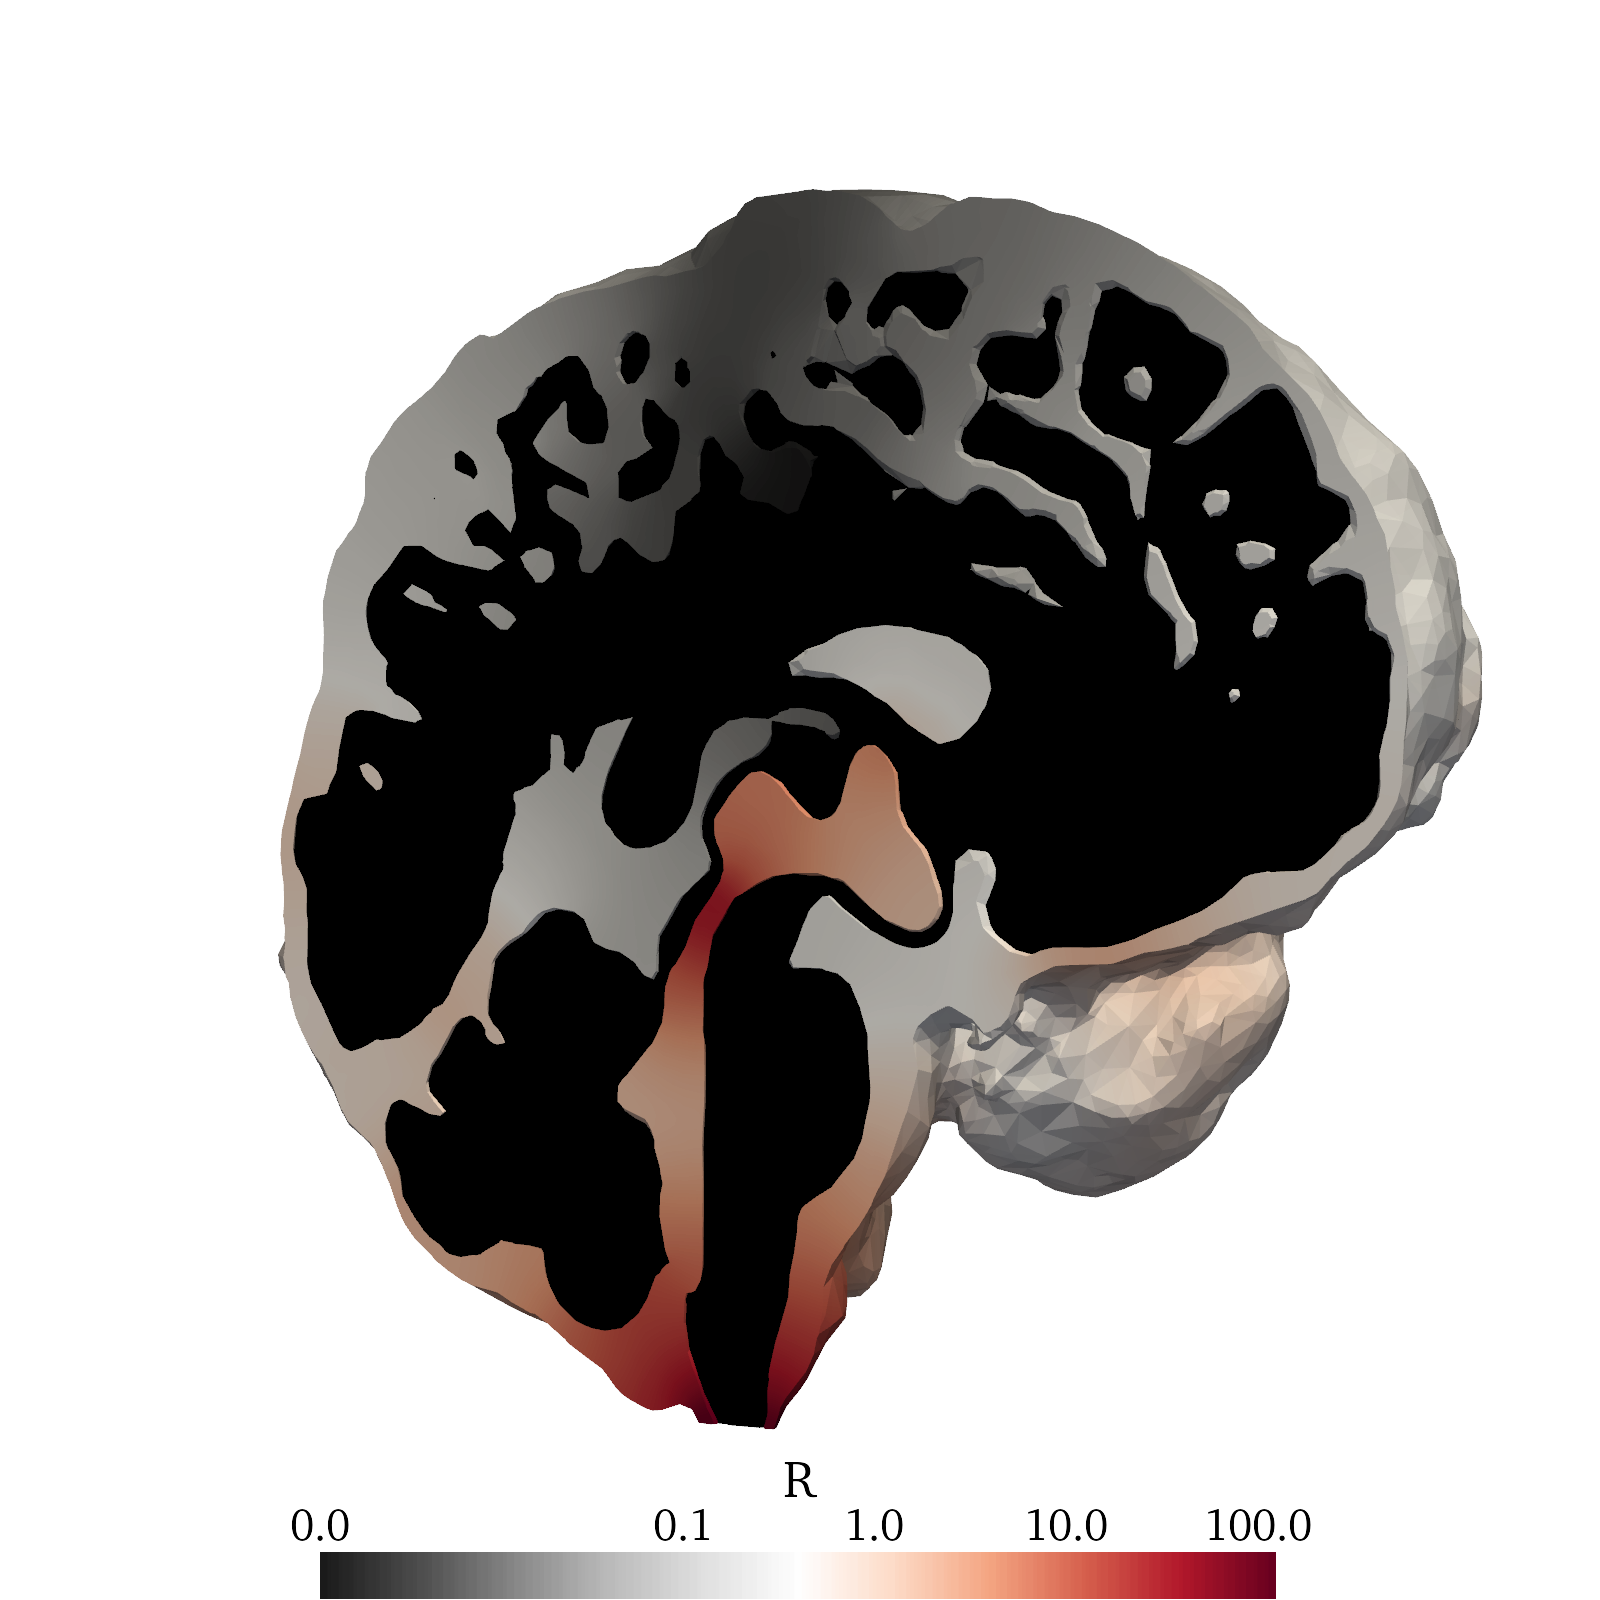
\includegraphics[width = 1 \textwidth]{figures/R.png} 
\caption{Dispersion enhancement factor $R$}
\label{fig:visualize_R}
\end{subfigure}
\caption{\mer{A) Illustration of 3D-domains; (B) Illustration of
    relevant boundaries; C) CSF flow induced by CSF production; D) CSF
    flow induced by peak arterial influx/peak volumetric influx of
    cardiac cycle; E) Computed dispersion factor.}}
\label{fig:csf}
\end{figure}  

\subsection*{III: Perivascular flow}

\draft{\lipsum[1]}

\begin{figure}
    \centering
    \begin{subfigure}[b]{0.33\textwidth}
    \centering
    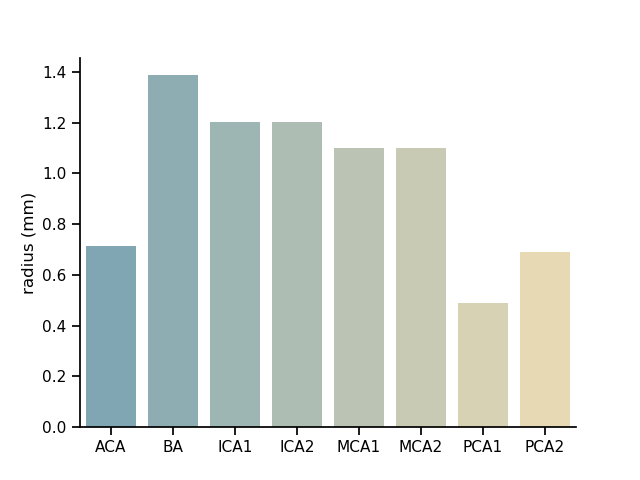
\includegraphics[width = \linewidth]{figures/arteries_labels_radius.png}
    \end{subfigure}
     \begin{subfigure}[b]{0.33\textwidth}
    \centering
    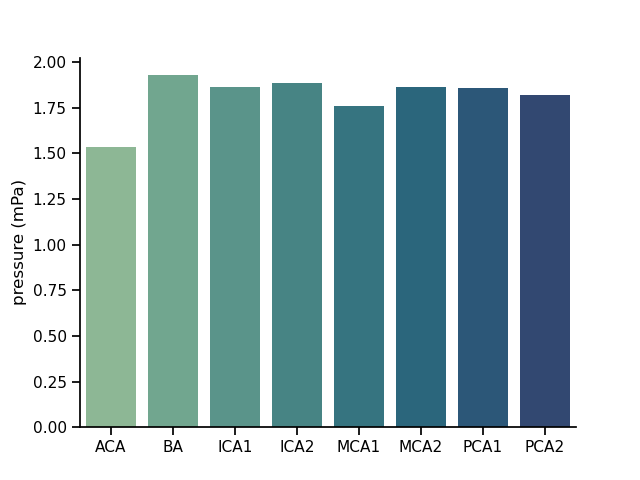
\includegraphics[width =  \linewidth]{figures/arteries_labels_pressure.png}
    \end{subfigure}
     \begin{subfigure}[b]{0.33\textwidth}
    \centering
    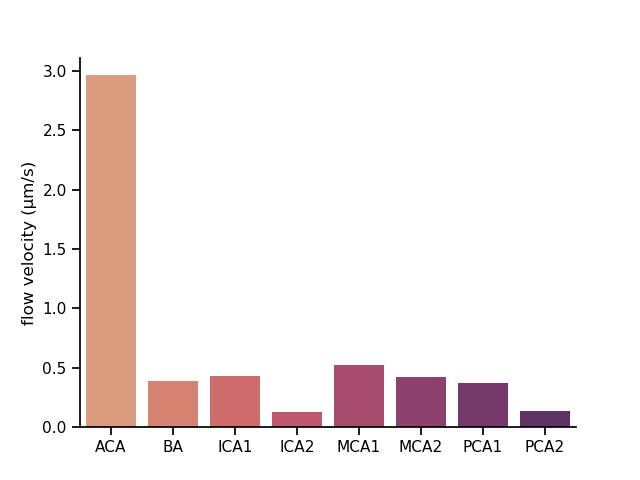
\includegraphics[width =  \linewidth]{figures/arteries_labels_velocity.png}
    \end{subfigure}
    \begin{subfigure}[b]{0.33\textwidth}
    \centering
    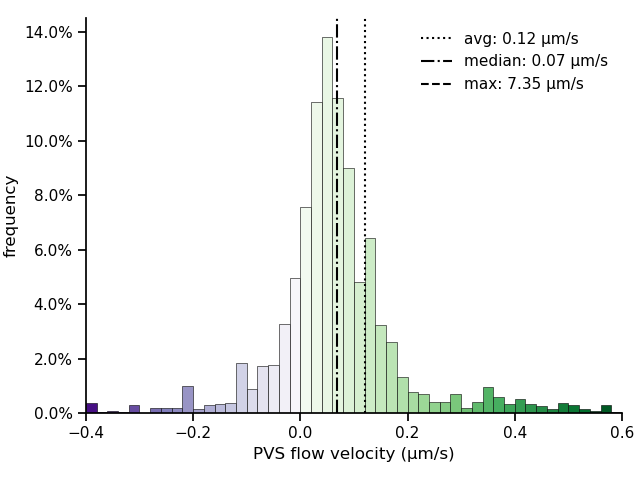
\includegraphics[width =  \linewidth]{figures/velocity_histo.png}
    \end{subfigure}
    %\label{fig:enter-label}
    \label{fig:pvs}
    \caption{\mer{MER: Put vasculature network illustration here. Many aspects actually. Marking of segments. Location relative to 3D. Radius etc. Marius will evaluate and suggest. Results: Group segments by logical order. For key arterial segments: average radius and length (can be moved to Supplementary if need be); pressure values; flow velocities; and then histograph with flow velocities for each mesh cell. Make sure to minorly note that ACA refers to a segment of the ACA and not the whole thing e.g.}}
\end{figure}

\Cref{fig:pvs}.

\subsection*{Structural versus functional compartmentalization of perivascular spaces}

\begin{itemize}
\item
  Are perivascular spaces functionally or structurally
  compartmentalized? Human and rodent observations indicate that
  tracers concentrate in perivascular spaces surrounding the pial and
  subarachnoid vasculature. Must these spaces be structural
  i.e.~defined by semi-permeable structural
  membrane~\cite{zhang1990interrelationships, zhang1992directional,
    mestre2018flow, eide2024functional}, or can such
  compartmentalization be a result of regions of enhanced flow or
  mixing~\cite{bedussi2017paravascular, vinje2021brain}? See also
  references in Background.
\item
  Compare Model A variations \Cref{tab:scenarios}).
\end{itemize}

\draft{\lipsum[1]}

\subsection*{The significance of low-resistance perivascular pathways}

\begin{itemize}
\item
  Perivascular flow and transport has been identified as a key
  mechanism and potential target for enhancing brain drug delivery and
  metabolic waste clearance -- what are the global (intracranial)
  effects of such intracranial highways? 
\item
  Compare Model A and B (\Cref{tab:scenarios}).
\item
  Do solutes move from PVS to the SAS, or both along the PVS and along the SAS?
\end{itemize}

\draft{\lipsum[1]}

\subsection*{Clearance and the brain's waterscape}

\draft{\lipsum[1]}

\begin{itemize}
\item 
  Modelling metabolite clearance rather than solute influx (Model
  C). Consider several diffusion coefficients corresponding to
  gadubutrol, dextran, tau and amyloid-beta, otherwise identical flow
  set-ups.
\end{itemize}

\subsection*{Intracranial solute influx and clearance during sleep}

\begin{itemize}
\item
  Sleep is known to affect a number of the transport characteristics including: increased extracellular volume fraction, altered vascular pulsatility and a-forteriori perivascular flow and mixing, reduced CSF production, reduced glymphatic transport.
\end{itemize}

\draft{\lipsum[1]}

\subsection*{Influx and clearance in pathologies}

\begin{itemize}
\item
  A number of neurological and neurodegenerative disorders yield mechanical changes in the intracranial environment (increased arterial stiffness, cerebral arterial angiopathies, perivascular flow changes due to hypertension, altered CSF flow patterns, altered diffusion properties in cancer, BBB leakage). One key clinical aspect is increased PVS width in e.g. iNPH. 
\end{itemize}

\draft{\lipsum[1]}



\iffalse
\newpage
\subsection*{Effect of interfaces (interface permeability)}

\begin{itemize}
    \item Model 0 (baseline): only diffusion, different diffusion coefficient in the parenchyma and SAS/PVS. No leak to vasculature (zero permeability). $\infty$ $\zeta_0$ at the PVS-SAS interface, $\zeta_1$ at the PVS-SAS interface. Koch et al could be a reference for PVS-parenchyma, maybe Tithof et al (2022, "A network model" ...) could give some ideas for parameters, also see Mestre et al, Nature comms, 2022. 
    \item 
    With altered interface permeabilities in the PVS (Model 1), and or in the parenchyma (Model 2) 
    \end{itemize}

\begin{figure}
    \caption{}
    \label{fig:1}
\end{figure}

\subsection*{Effect of convection}
\begin{itemize}
    \item 
    With convective flow in the PVS (zero flow in the parenchyma for now)
    \begin{itemize}
        \item 
        Model 3: PVS flow equal to 18.7 $\mu$m/s
        \item 
        Model 4: Better PVS flow (distributed, according to conservation of mass, assumptions on PVS area)
    \end{itemize}    
    \item 
    With convective flow in the ECS (out of scope here, for follow-up work?)
\end{itemize}

\begin{figure}
    \centering
    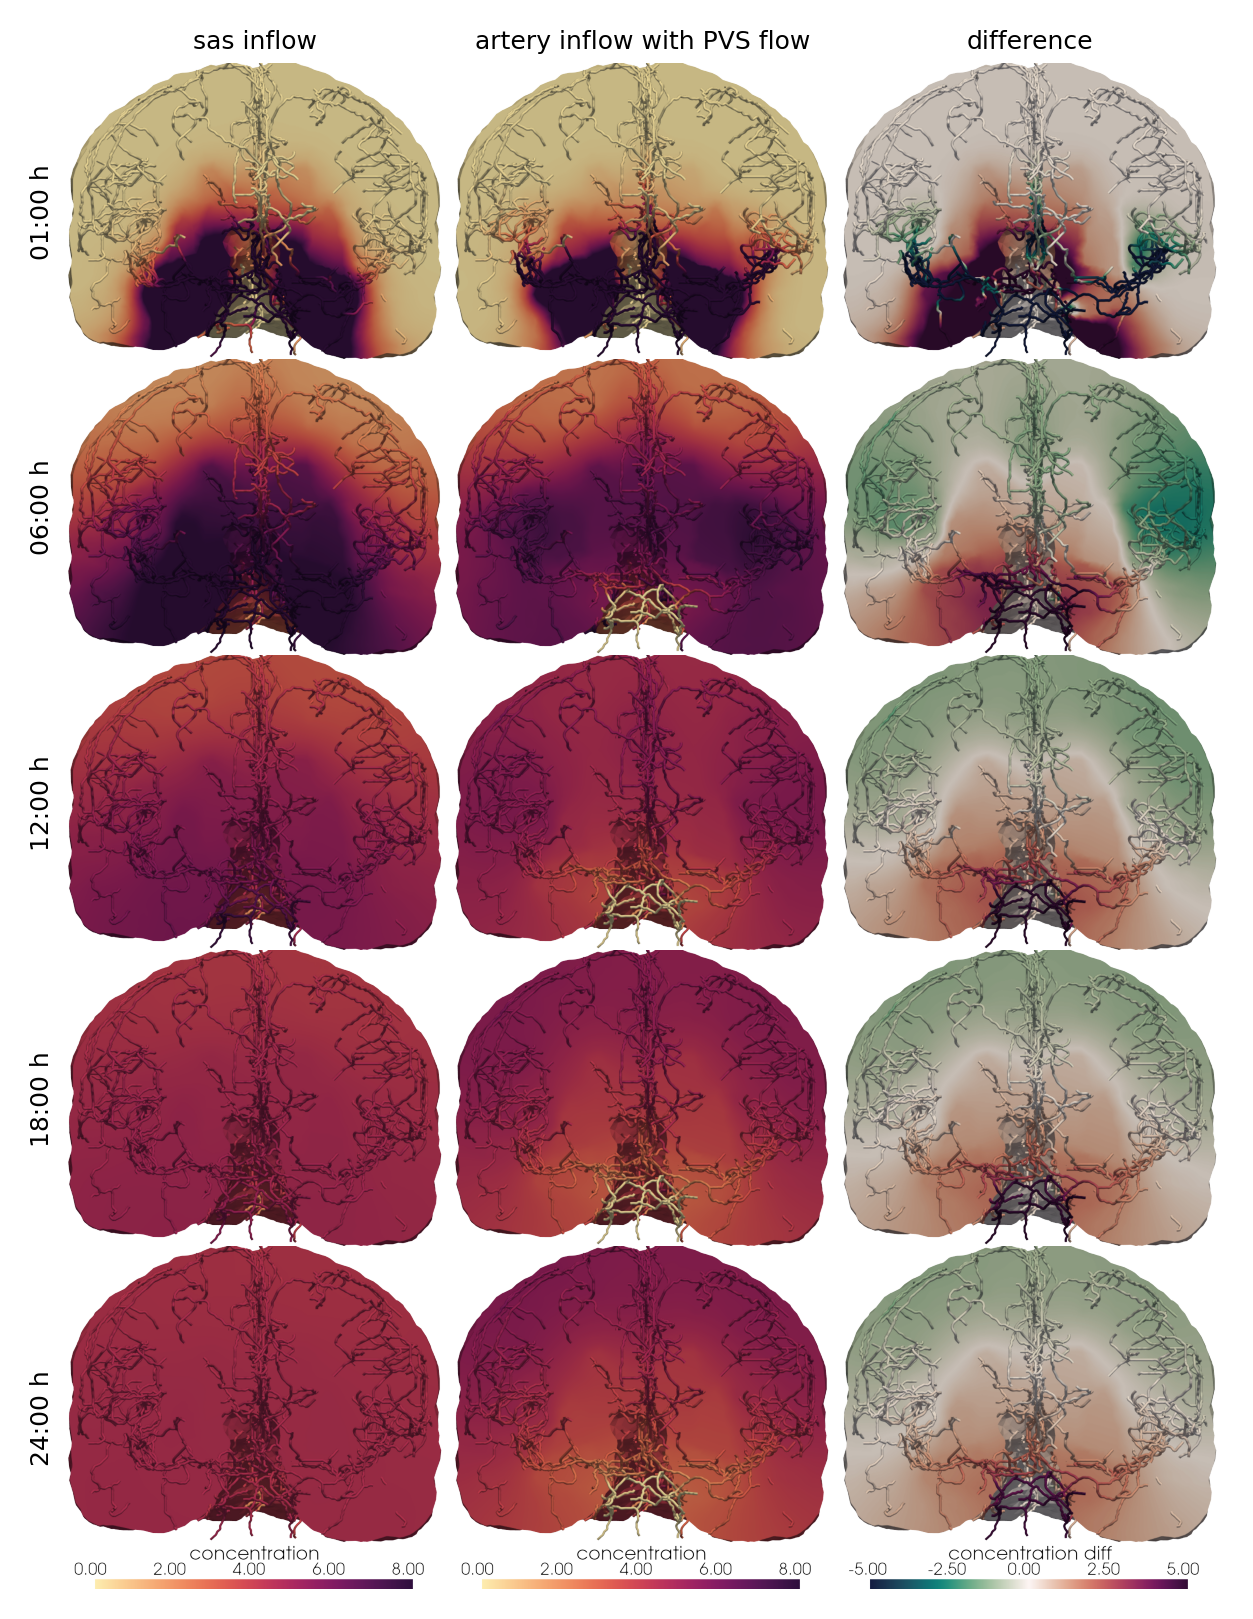
\includegraphics[width = 0.9 \textwidth]{modelB_modelC_overview.png}
    \caption{Tracer concentrations for a purely diffusive model with tracer inflow via the CSF-filled space (left) and a convective model with Tracer inflow via the arterial PVS (middle) and their difference (right) at 1, 6, 12, 18 and 24 hours after injection.}
    \label{fig:2}
\end{figure}
\subsection*{Effect of BBB}

Leakage to the blood, some sink/non-zero permeability for the PVS-blood (BBB) interface (Model N).

\begin{figure}
    \caption{}
    \label{fig:3}
\end{figure}

\subsection*{Effect of pia}
  
Effect of pia permeability (Model N-1)    

\begin{figure}
    \caption{}
    \label{fig:4}
\end{figure}

\begin{figure}
     \centering
     \begin{subfigure}[b]{0.33\textwidth}
         \centering
         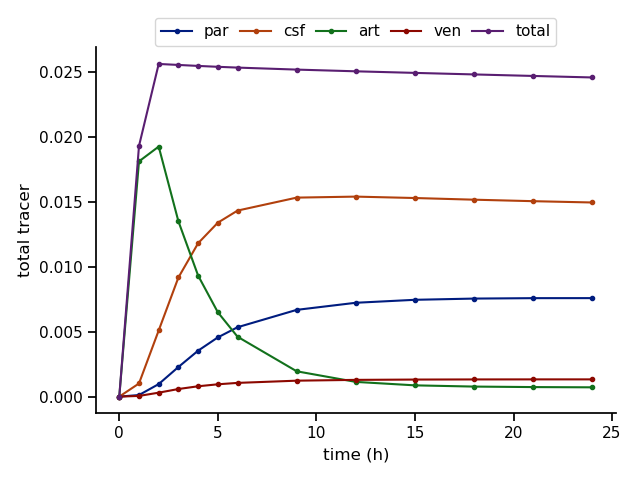
\includegraphics[width=\textwidth]{modelA_total_conc.png}
         \caption{arterial inflow, pure diffusion}
         \label{fig:y equals x}
     \end{subfigure}
     \hfill
     \begin{subfigure}[b]{0.33\textwidth}
         \centering
         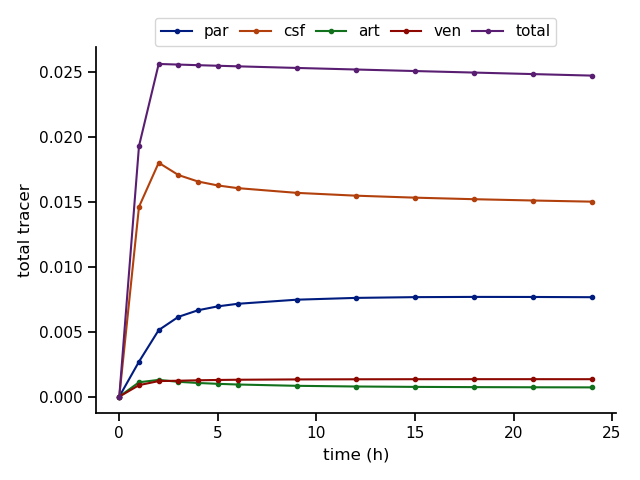
\includegraphics[width=\textwidth]{modelB_total_conc.png}
         \caption{SAS inflow, pure diffusion}
         \label{fig:three sin x}
     \end{subfigure}
     \hfill
     \begin{subfigure}[b]{0.33\textwidth}
         \centering
         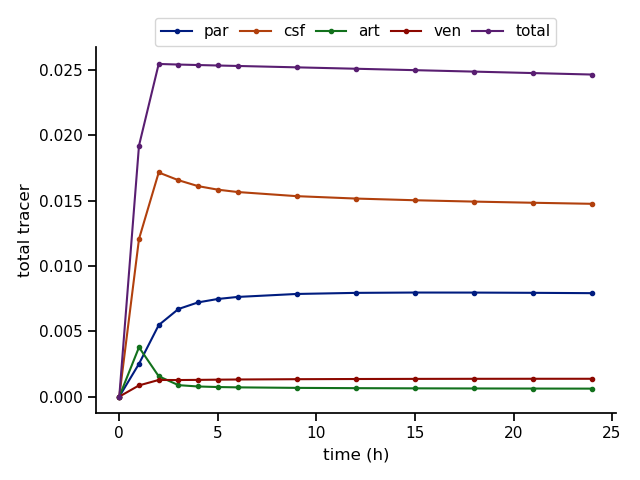
\includegraphics[width=\textwidth]{modelC_total_conc.png}
         \caption{arterial inflow, diffusion + PVS convection}
         \label{fig:five over x}
     \end{subfigure}
        \caption{Total tracer amount in parenchyma, CSF, arterial PVS and venous PVS}
        \label{fig:three graphs}
\end{figure}

\fi

\newpage
%%%%%%%%%%%%%%%%%%%%%%%%%%%%%%%%%%%%%%%%%%%%%%%%%%%%%%%%%%%%%%%%%%%%%%%%%%%%%%%%%%%%%
\section*{Methods}

%\mer{MER: I recommend writing each (sub)section of Methods as a nearly stand-alone paragraph. Let's see if we can avoid subsubsections/paragraphs. If you need to add more detail than you think is appropriate, put it in a Supplementary Methods section in the Appendix.} 

\subsection*{Brain parenchyma, SAS, and interface geometries}


Hodneland et al~\cite{hodneland2019new} developed a method to image
the brain's microvasculature based on time-of-flight (ToF) and
quantitative susceptibility mapping (QSM) to identify arterial and
venous networks.  We derive a detailed tetrahedral mesh of the
parenchyma and the surrounding CSF-filled spaces alongside a network
representation of the vasculature from the anatomical data provided
therein. 

First, we segment the structural T1 image using Synthseg \cite{billot2023robust,billot2023synthseg} to obtain masks of the parenchymal tissue and the CSF-filled spaces. In addition, we slightly modify the segmentation to ensure correct connectivity of the ventricular system. In particular, we elongate the aqueduct and enforce no communication between the ventricles and the surrounding CSF spaces except for the median aperture. After morphological smoothing of the segmented image, we extract surface representations of the outer SAS boundary, the pial membrane and the components of the ventricular system. From these surface representations, we create a tetrahedral mesh of both the parenchymal tissue and the CSF-filled spaces using the mesh generator fTetWild \cite{hu2020fast}. The resulting mesh consists of 153729 vertices and 851904 cells, which vary between $0.4$\,mm and $1.2$\,cm in cell diameter. The parenchyma has a total volume of $1386$\, ml, whereas the ventricles and the outer SAS contribute $28$\,ml and $277$\,ml to a total CSF volume of $305$\,ml, respectively. Note that the widely reported value of $150$\,ml of intracranial CSF volume is likely an underestimate. Recent estimates indicate that a value of $200$ to $300$\,ml is more accurate (see \cite{hladky2024regulation} and references therein).
\mar{this could also go into results. Keep it here for the moment?} \mer{I suggest you place the ``note'' in the Discussion.}


The computational domain $\Omega$ is defined by the union of the CSF spaces $\Omega_{\rm CSF}$ and brain parenchyma $\Omega_{\rm PAR}$ (\Cref{fig:concept}). The thin pia membrane encloses the brain, and we hence denote the CSF-brain interface with $\Gamma_{\rm pia}$, except for the separately marked surface of the lateral ventricles $\Gamma_{\rm LV}$ (thus $\partial \Omega_{\rm CSF} \bigcap \partial \Omega_{\rm PAR} = \Gamma_{\rm LV} \cup \Gamma_{\rm Pia}$).

We denote the different parts of the outer boundary of $\Omega_{\rm CSF}$ with
$\Gamma_{\mathrm{skull}}$ facing the dura and skull and $\Gamma_{\rm SSAS}$ representing the lower interface towards the spinal subarachnoid space (SSAS). $\Gamma_{\mathrm{skull}}$ is further subdivided into its lower and upper parts: $\Gamma_{\mathrm{skull^l}}$ and $\Gamma_{\mathrm{skull^u}}$ (compare \Cref{fig:concept}). The boundary of the spinal cord is denoted by $\Gamma_{\rm{SC}}$, which is given by $\Gamma_{\rm{SC}} = \partial \Omega_{\rm PAR} \setminus \partial \Omega_{\rm CSF}$ .

\subsection*{Vascular and perivascular domains and networks}

\mer{Is this up-to-date? @Rami checks sanity and numbers of paragraph.}

We skeletonize the binary masks of the arteries and veins of the
Hodneland~\cite{hodneland2019new} data set using
Kiminaro~\cite{william_silversmith_2021_5539913}, to obtain the
centerline $\Lambda^i$ and radius $R_1^i$ of each detected vessel $i$,
and the vessel connections. The resulting vascular networks are
further smoothened using a spline interpolation technique, and
represented as graphs with nodes connected by edges. The arterial
network contains 11862 nodes (and 11861 edges), while the venous
network contains 21883 nodes (and 21882 edges); with no cycles in
either network. Nodes connected to only one edge (i.e.~with graph
degree 1) are labeled terminal nodes. For the arterial network, we
identify 3 of the terminal nodes, representing \mer{the two internal
  carotid arteries and the basilar artery}, as root nodes
(\Cref{fig:concept}) and label the other terminal nodes as leaf
nodes. \mer{Range of lengths of the networks paths.} We denote the
domain defined by the connected centerlines by $\Lambda$. The vascular
domain is then represented as the union of cylindrical vessels of
radius $R_1^i$ surrounding the centerlines $\Lambda^i$. Moreover, we
consider the surrounding perivascular spaces as the union of annular
cylinders of inner radius $R_1^i$ and outer radius $R_2^i = \beta R_1^i$ of width $R_2^i - R_1^i = (\beta - 1) R_1^i$. Both the vasculature and perivasculature are thus defined relative to a common network of vessel segments.


\begin{figure}
     \centering
     \begin{subfigure}[b]{0.45\textwidth}
         \centering
         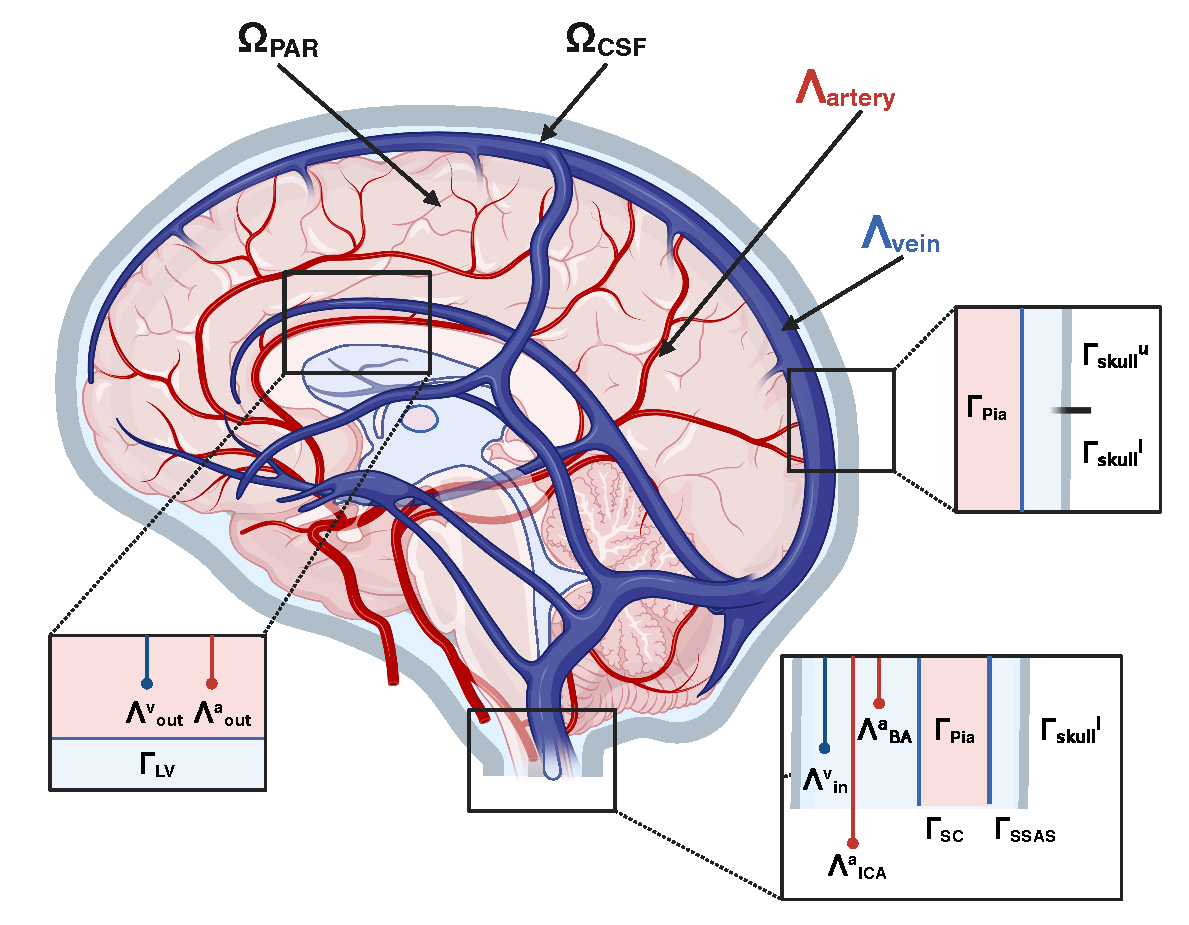
\includegraphics[width=\textwidth]{figures/Brain-PVS-callouts.pdf}
         \caption{Concept sketch}
         \label{fig:y equals x}
     \end{subfigure}
     \hfill
     \begin{subfigure}[b]{0.3\textwidth}
         \centering
         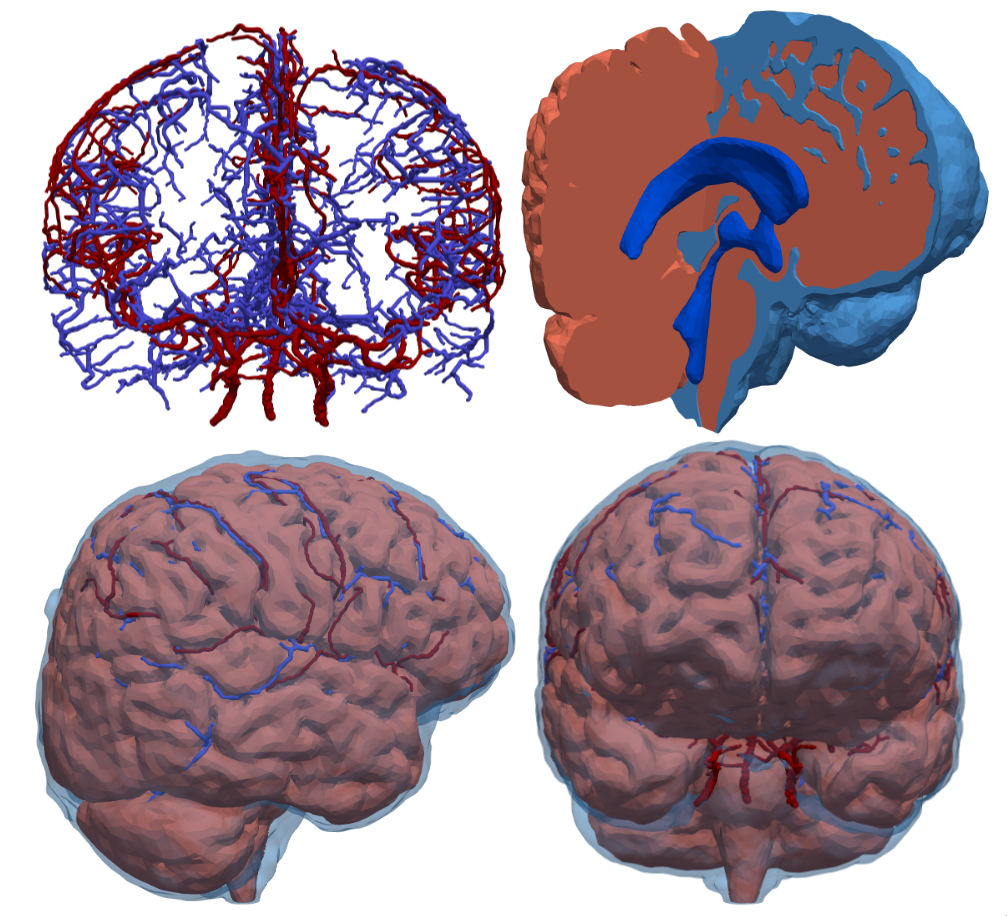
\includegraphics[width=\textwidth]{figures/geometry_concept.png}
         \caption{The arterial (red) and venous (blue) networks (top left), the parenchyma and CSF space (top right), combined (bottom row)}
         \label{fig:three sin x}
     \end{subfigure}
     \hfill
     \begin{subfigure}[b]{0.24\textwidth}
         \centering
         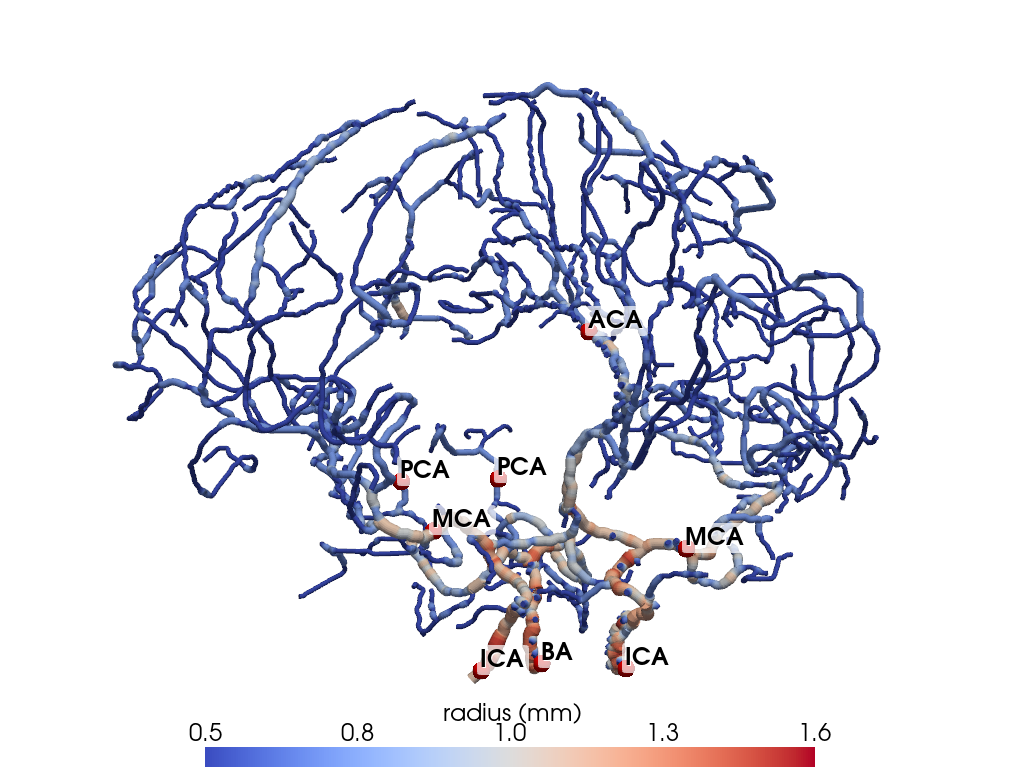
\includegraphics[trim={4cm 0 4cm 0},clip,width=\textwidth]{figures/labeled_arteries.png}
         \caption{The arterial network with the main cerebral arteries: internal carotid artery (ICA), middle cerebral artery (MCA), anterior cerebral artery (ACA) and posterior cerebral artery (PCA)}
         \label{fig:five over x}
     \end{subfigure}
  \caption{@Marius: Starts adding parts of this. \mer{MER: Concept figure illustrating the compartments and story line. (A) Concept sketch of the SAS, PVS and the brain; (B) Visualization of geometry domains (brain, sas and vasculature; think about colors and associations; please don't make blood blue and water red e.g.) ; (C) Zoom-in/detail on vasculature, which are which arteries (ACA, MCA, PCA, CoW)  and veins (XXX); (D) Zoom-in 2 on vascular position versus SAS and brain; (E) Zoom-in 3 on where PVS ends; (F) Illustration of boundaries? (G) Concept illustration of the mathematical model (diffusion, convection, exchange, boundaries).}}
\label{fig:concept}
\end{figure}

\subsection*{Multi-dimensional intracranial transport equations}

We model diffusion, convection and exchange of a solute in PVSs, in the surrounding SAS and in the brain parenchyma (Fig.~\ref{fig:concept}) via a comprehensive multi-dimensional transport model~\cite{masri2023modelling} over a timescale of minutes to hours. More specifically, we solve for a solute concentration $c$ defined locally in each subdomain $c = c_{\rm{csf}}$ in $\Omega_{\rm{csf}}$ and $c =c_{\rm{PAR}}$ in $\Omega_{\rm{PAR}} $, 
and for an averaged solute concentration $\hat c$ in a 1D network of centerlines $\Lambda$ representing the PVS ($\hat c$ defined locally on each $\Lambda^i$), such that the following equations hold
\begin{subequations}
\begin{alignat}{2}
  \partial_t (\phi c) - \nabla \cdot (D \nabla (\phi c) ) + \nabla \cdot (\bm u c ) + \xi (\overline{c} - \hat c ) \delta_\Gamma & = f && \quad \quad \mathrm{in} \quad \Omega_{\rm CSF} \cup \Omega_{\rm{PAR}}, \label{eq:multi_transport_3d} \\ 
  \partial_t (A  \hat c) - \partial_s(\hat D A \partial_s ( \hat c)) +\partial_s(A \hat u \hat c )  +  \xi P (\hat c - \overline{c})  &= A \hat f && \quad \quad \mathrm{in} \quad  \Lambda . \label{eq:multi_transport_1d}
 \end{alignat}
\end{subequations}
The notation $\overline{c}$ denotes the lateral average of the concentration over the outer perivascular boundary \footnote{
The lateral average is defined as 
\[ \overline{c}(s) = \frac{1}{A(s)} \int_{\Theta(s)} c ,\]
where $\Theta(s)$ is a cross-section of the PVS at the point on $\bm{\lambda}(s)$ on $\Lambda$ where $\bm \lambda$ is a given parameterization of $\Lambda$ and $A(s)$ is the area of $\Theta(s)$. 
}. The (Dirac delta) term $\delta_\Gamma$ is a source term concentrated on the outer boundary of the PVS (the union of the annular domains surrounding $\Lambda^i$) that models the solute exchange between the PVSs and their surroundings \footnote{The term $\delta_{\Gamma}$ is given for any function $v$, see \Cref{sec:details_numerical_method} for more details
\[\xi  (\overline{c} - \hat c ) \delta_\Gamma (v) 
= \int_{\Lambda} P \xi ( \overline{c} - \hat c ) \overline{v} 
\]
}.  
Here $\phi$ is the fluid volume fraction (or porosity) of the brain (where $\phi \ll 1$), of the SAS (where $\phi = 1$) and of the PVS (where $0 \ll \phi \leq 1$); $D$ is the effective diffusion coefficient of the relevant solute in the respective media~\cite{sykova2008diffusion} which takes different values over the SAS and brain,  $\bm u$ and $\hat u$ are convective velocity fields in $\Omega$ and $\Lambda$ respectively, and $\xi$ is a transfer coefficient across the PVS-CSF and the PVS-Brain interface
\[
\phi =  \begin{cases}
    1  & \mathrm{in} \;  \Omega_{\rm{csf}} \\ 
    \phi_{\rm{PAR}} & \mathrm{in} \; \Omega_{\rm{PAR}} 
    \end{cases}, \; 
 D= \begin{cases}
    D_{\rm{csf}} & \mathrm{in} \;  \Omega_{\rm{csf}} \\ 
    D_{\rm{PAR}} (1+ R) & \mathrm{in} \; \Omega_{\rm{PAR}} \end{cases}, \; 
    \quad \bm u  = \begin{cases}
    \bm{u}_{\rm{csf}} & \mathrm{in} \; \Omega_{\rm{csf}} \\ 
    \bm{u}_{\rm{PAR}} & \mathrm{in} \; \Omega_{\rm{PAR}} 
\end{cases}, \; 
\xi = \begin{cases}
 \xi_{\rm{PVS}, \rm{PAR}} & \mathrm{if} |\Lambda^i \cap \Omega_{\rm{PAR}}| \neq 0 \\ 
  \xi_{\rm{PVS}, \rm{csf}} & \mathrm{if} |\Lambda^i \cap \Omega_{\rm{csf}}| \neq 0
\end{cases} . 
\]
We refer to \Cref{tab:overview} for the values of the used parameters.
In the above,  $|\Lambda^i \cap \Omega_{\rm{PAR}}|$ (resp.  $|\Lambda^i \cap \Omega_{\rm{csf}}|$) is nonzero whenever the surrounding PVS around the line $\Lambda^i$ intersects $\Omega_{\rm{PAR}}$ (resp. $\Omega_{\rm{csf}}$). If the surrounding PVS intersects both, then we set $\xi = \xi_{\mathrm{PVS}, \rm{PAR}}$ (resp $\xi_{\mathrm{PVS}, \rm{PAR}}$) if the PVS lies mostly ($80$ percent) in $\Omega_{\rm{PAR}}$ (resp. $\Omega_{\rm{PVS}}$) and the interaction with $\Omega_{\rm{PVS}}$ (resp. $\Omega_{\rm{PAR}}$ is ignored. 

Further, $P$ and $A$ are the perimeter and area of the PVS which can vary along the centerline network, respectively; and $f$ and $\hat{f}$ represent given sources of solute in $\Omega$ and $\Lambda$, respectively. Finally, we remark that $\hat u$ takes different values on each $\Lambda_i$.  Both $\Omega$ and $\Lambda$ are fixed in time here. Finally, we note that this version of the model assumes that there is no interaction between the inner perivascular boundary and the blood vessel. 

%\noindent \mer{MER: @Rami: I've added the $\phi$'s in this subsection. Please review and add convective terms in $\Omega$ and $\Lambda$.} \rami{done, maybe I include a more precise variational formulation in the appendix ? }
\subsubsection*{Initial conditions}

We set the initial concentrations $c_0, \hat{c}_0$ in the three-dimensional domain $\Omega$ and network $\Lambda$ to be zero for all influx scenarios (Models A--\draft{X-1}). For modelling clearance (Model \draft{X}), we set $c_0 = 1, \hat{c}_0 = 0$.

\subsubsection*{Boundary conditions: extracranial efflux and perivascular parenchymal influx}
On the interface $\Gamma_{\mathrm{pia}}$ between the CSF and brain, we prescribe the following condition modeling a semi--permeable pial interface 
\begin{alignat}{2}
(-D \nabla (\phi c_{\rm{PAR}}) + \bm u_{\rm{PAR}} c_{\rm{PAR} }) \cdot \bm{n}_{\rm{PAR}} &= - (- D \nabla c_{\rm{CSF}} + \bm u_{\rm{CSF}} c_{\rm{CSF}} ) \cdot \bm{n}_{\rm{PAR}} &&  \quad  \mathrm{on} \quad \pia \cup \Gamma_{\mathrm{LV}} ,  \\  
(-D \nabla ( c_{\rm{PAR}}) + \bm u_{\rm{PAR}} c_{\rm{PAR} }) \cdot \bm{n}_{\rm{PAR}} & = \beta_{\rm{pia}} (c_{\rm PAR} - c_{\mathrm{CSF}}) &&  \quad  \mathrm{on} \quad  \pia \cup \Gamma_{\mathrm{LV}} .  
\end{alignat} 
Here, $\beta_{\mathrm{pia}}$ is a permeability constant between the brain and the CSF: On $\Gamma_{\mathrm{skull}}$, the interface towards the dura and skull (\Cref{fig:concept}), we consider a constant uptake (or efflux) rate, represented by the boundary condition 
\begin{alignat}{2}
(- D \nabla ( c_{\mathrm{CSF}}) + \bm u_{\mathrm{CSF}} c_{\mathrm{CSF}}) \cdot \bm{n}   & = \beta c_{\mathrm{CSF}}  && \quad \mathrm{on} \quad \Gamma_{\mathrm{skull}^{\rm u}},\\ 
(-D \nabla c_{\rm CSF} + \bm u c_{\rm CSF}) \cdot \bm{n} & =  0   &&  \quad  \mathrm{on} \quad \Gamma_{\rm skull^{l}} , 
\end{alignat}
where $\beta$ represents a molecular outflow resistance. Here, we take $\beta = 10^{-4} \,\, \mathrm{mm}^2/\mathrm{s}$\cite{hornkjol2022csf}.
\mer{Marius says that this $\beta$ makes the solute accumulate. Maybe we want to modify this parameter.}

Modelling an intrathecal injection, we prescribe a time-dependent solute influx rate on the interface towards the spinal compartment $\Gamma_{\mathrm{SSAS}}$
with the condition 
\begin{alignat}{2}
    (D \nabla  c_{\mathrm{csf}} - \bm u_{\mathrm{csf}}c_{\mathrm{csf}} ) \cdot \bm{n}_{\spinal} & = g_{\mathrm{influx}} &&   \quad  \mathrm{on} \quad \spinal  \end{alignat}
Here, we set
\begin{equation}
g_\mathrm{influx}(t) = \frac{m_{\rm tot}}{T_{\rm max}^2 |\Gamma_{\rm SSAS}|} \max(0, T_{\rm max} - |t - T_{\rm max}|)
\end{equation}
which results in a triangular inflow function with a peak at $T_{\rm max} = 3600\,$s and a total tracer injection of $m_{\rm tot} = 0.5$\,mM.

For the perivascular network, the boundary nodes are collected into $\partial \Lambda$. We assume no tracer outflow on all boundary nodes and prescribe a homogeneous Neumann condition: 
\begin{equation}
    \hat D A \partial_s (\phi \hat c) - A \hat u \hat c  = 0 \quad \mathrm{on} \quad \partial \Lambda. 
\end{equation}
For bifurcation nodes, we impose flux conservation and continuity of the concentration $\hat c$. We refer to \eqref{eq:flux_conservation} in \Cref{sec:details_numerical_method} for more details. 

\subsection{Cerebrospinal fluid flow in the subarachnoid space} \label{sec:csf_fluid_vel}

We consider non-zero convection in the CSF space $u_{\rm CSF} \not = 0$ in \eqref{eq:multi_transport_3d} resulting from steady state CSF production.  Recall that $\Omega_{\mathrm{CSF}}$ represents the CSF space and that $\Gamma_{\mathrm{skull^{u/l}}}$ and $\Gamma_{\mathrm{pia}}$, $\Gamma_{\mathrm{LV}}$ represent the boundaries facing the upper and lower parts of the dura, the pia and the lateral ventricles, respectively.  Assuming CSF production in the choroid plexus located at the lateral ventricle wall, we solve the  steady state Stokes equations for the velocity and the pressure $(\bm u_{\mathrm{CSF}}, p_{\mathrm{CSF}})$ in the CSF domain: 
\begin{subequations}
    \begin{alignat}{2}
 - \mu \Delta \bm u_{\mathrm{CSF}} + \nabla p_{\rm{CSF}} & =  0 \quad && \mathrm{in} \,\,  \Omega_{\rm CSF}, \label{eq:momnetum_equation}  \\ 
 \nabla \cdot  \bm u_{\mathrm{CSF}} & = 0 \quad && \mathrm{in} \,\,   \Omega_{\rm CSF}, \label{eq:divergence_equation}  \\ 
\mu \nabla \bm u_{\mathrm{CSF}} \cdot \bm{n} -  p \bm n  &  = -R_0 ( \bm u \cdot \bm n ) \bm n\,\,   && \mathrm{on}  \label{eq:efflux_condition} \,\, \Gamma_{\mathrm{skull^u}}, \\ 
\bm u_{\mathrm{CSF}} & = 0 && \mathrm{on} \,\, \Gamma_{\rm{pia}} \cup \Gamma_{\mathrm{skull^l}} \Gamma_{\rm{SSAS}}  \\
\bm u_{\mathrm{CSF}} \cdot \bm n & = u_{\rm in} / |\Gamma_{\rm LV}| && \mathrm{on} \,\, \Gamma_{\rm{LV}} .  
\end{alignat}
\end{subequations}

Here, $\bm n$ denotes the unit outward normal to the boundary, $\mu$ is the CSF viscosity, and $u_{\rm in}$ is the steady CSF flow across the lateral ventricle wall. Condition \eqref{eq:efflux_condition} models an efflux site with positive resistance $R_0 \geq 0$. The Stokes system is solved with the finite element software $FEniCS$, stored and then subsequently read for all the relevant solute transport simulations. See Figure~\ref{fig:csf_flow_cardiac} for a streamline visualization of the obtained velocity profile and \Cref{sec:details_numerical_method} for details on the numerical algorithm employed.



\subsection*{Dispersion induced by pulsatile fluid flow in CSF spaces}

With each cardiac and respiratory cycle, CSF pulsates in the ventricular system and the subarachnoid space. Sharp et al \cite{keith2019dispersion} estimated the enhancement of diffusion in the spinal subarachnoid space due to dispersive effects to average 5.8 times that of purely molecular diffusion with a theoretical maximum of $10^6$. Taking the large spatial differences of pulsatile CSF flow into account, we compute the local diffusion enhancement factor $R$ in the CSF-filled space $\Omega_{\rm CSF}$ by combining a computational model of cardiac induced CSF flow with theoretical estimates for shear-augmented (Taylor) dispersion \cite{taylor1953dispersion, watson1983diffusion}.

Similar to the case of CSF flow driven by production introduced in section \ref{sec:csf_fluid_vel}, we employ a Stokes flow model to predict CSF velocities at peak arterial dilation. In particular, we enforce a uniformly distributed inflow of $10$\,ml/s and $2$\,ml/s across the outer skull ($\Gamma_{\rm skull}$) and lateral ventricular surfaces ($\Gamma_{\rm LV}$) respectively, mimicking the effect of reduced CSF volume due to blood inflow. We prescribe a no-slip boundary condition on the pial surface $\Gamma_{\rm Pia}$ and zero-traction on the spinal boundary $\Gamma_{\rm SSAS}$, making the spinal compartment the only outflow route of CSF. Thus, we compute the cardiac-driven flow field by augmenting the Stokes flow model (eq. \ref{eq:momnetum_equation} and \ref{eq:divergence_equation}) with the following boundary conditions:

\begin{equation}\label{eq:cardiac_flow_bcs}
    \bm u = 0 \text{ on } \Gamma_{\rm Pia}; \quad 
    \mu \nabla \bm u \cdot \bm n - p \bm n = 0 \text{ on } \Gamma_{\rm SSAS}; \quad 
    \bm u = \frac{0.31 \cdot \bm n}{|\Gamma_{\rm LV}|} \,\text{ml/s} \text{ on } \Gamma_{\rm LV}; \quad
    \bm u = \frac{8 \cdot \bm n}{|\Gamma_{\rm skull}|} \,\text{ml/s} \text{ on } \Gamma_{\rm skull}.
\end{equation}

The obtained pressure field only account for viscous forces, albeit cardiac induced CSF flow is known to be unsteady and substantially impacted by transient inertial forces. Assuming an oscillatory flow with the heartbeat frequency $\omega = 2 \pi$, a mean gap width of the CSF-filled spaces of $2h=3$\,mm and CSF density $\rho=10^3\,\text{kg/m}^3$, the Womersley number $\alpha$ becomes $\alpha^2 = \frac{h^2 \omega \rho}{\mu} = 20.2$, which is unsteady. Based on theoretical considerations on the ratio of oscillatory flow to steady flow impedances in a tube, we account for inertial forces in the pulsatile flow by upscaling the computed viscous pressure field by a factor of $1 + \alpha^2 / 8$ (see \cite{van1998cardiovascular}, chapter. 4.3).

Further assuming unsteady dispersion, we follow Sharp et al \cite{keith2019dispersion} and calculate the enhancement factor $R$ from the non-dimensionalized pressure gradient $dP=\frac{|\nabla p|}{\omega \mu / h}$ as $R\approx dP^2 / \alpha^3$. Combining the computed pressure gradient with this scaling law yields a pointwise approximation of the dispersion factor. Finally, we account for the non-local nature of the dispersion mechanism by applying a smoothing technique to obtain a spatially varying, but locally averaged diffusion enhancement factor $R$ (see the visualization in \cref{fig:visualize_R} and \cref{sec:dispersion_details} for additional details).


\subsection*{Cerebrospinal fluid flow in the perivascular spaces}
\label{sec:csf_pvs}
We obtain the fluid velocity $\hat u = \hat u_{\rm prod}$  in \eqref{eq:multi_transport_1d} by averaging the tangential component of $\bm u_{\mathrm{sas}}$ locally on each centerline $\Lambda_i$. Precisely, for all $i$ we compute 
\begin{equation}
\hat u_{\rm {prod}}(s) = \frac{1}{A(s)} \int_{\Theta(s)} \bm u \cdot \bm \tau_i, \quad \mathrm{in} \,\,  \Lambda_i.   
\end{equation}
 In the above $\bm u$ evaluates to $\bm u_{\rm{sas}}$ on $\Omega_{\rm CSF}$ and to zero otherwise, $\bm \tau_i$ is the tangent vector determined by the centerline $\Lambda_i$, $\Theta(s)$ is the cross-section of the PVS point at point $s$ and  $A$ is the area of this cross-section. \rami{to place a visualization here too }

\subsection*{Fluid flow within the parenchyma}
\label{sec:csf_brain}

We assume no significant convection in the brain $\Omega_{\rm PAR}$, and set $u = u_{\rm PAR} = 0$ there as a first approximation. 

\subsection*{Numerical approximation of multi-dimensional transport and CSF flow}

\mer{@Rami: Could you draft one paragraph here describing the essential bits of the numerical scheme? I recommend ``describing with words'' to reach relevant audiences. Refer to the Supplementary Methods for details. Mention theoretical expected convergence order.} 

In this section, we provide a brief overview on the employed numerical discretization. We refer to \Cref{sec:details_numerical_method} for detailed expositions on the approximation. The numerical scheme for the CSF flow equations utilizes polynomial spaces that preserve the divergence free condition \eqref{eq:divergence_equation} on the discrete level \cite{hong2016robust}. This requirement is important for stability in the transport equation, see for example \cite{cesmelioglu2022compatible}. The spaces we used for the velocity are continuous along the normal direction; continuity of the tangential component is enforced via interior penalty approaches \cite{hong2016robust}.  If the true solution is smooth, then one expects optimal error convergence rates for the aforementioned methods.

For the 3D transport problem, we use the interior penalty discontinuous Galerkin (DG) method with weighted averages and upwinding for the convection term \cite{ern2009discontinuous}.  We remark that the choice of DG is necessary here since  continuous Galerkin methods even when supplemented with streamline upwind stabilization are completely unstable. For the 1D transport problem, we use continuous Galerkin spaces defined over the entire network with additional streamline upwind Petrov–Galerkin stabilization when the 1D velocity is non--zero.  DG methods for the coupled 3D--1D problem have been recently analyzed  where convergence of the method for the elliptic case is established \cite{masri2024discontinuous}. While the analysis is for DG methods for both the 3D and the 1D problem, we expect similar arguments to hold here. However, note that the 3D--1D coupling induces a singularity in the 3D solution and one can only expect suboptimal error rates near the 1D network. In subdomains excluding the 1D lines, almost optimal rates can be expected for both DG methods \cite{masri2023discontinuous} and CG methods \cite{koppl2016local}.  Extension of the convergence to convection--diffusion problems is an interesting future research direction. 
 

\subsection*{Implementation and numerical verification}

\mer{@Miro: 2-3 sentences on the implementation.}

\mer{We need to demonstrate that our ``quantities are converged'', meaning we have a feel for how accurate our results are in practice (e.g.$\pm$ 1\%, 10\%, 100\%, 1000\%). Refer to the Supplementary table for a numerical verification table (quantities of interest versus mesh and time refinement for pure diffusion and one case with convection). Not on top of list of priorities, but not on bottom either.} 

\begin{enumerate}
\item
  Examine ``practical convergence'' of the CSF flow field. Three
  different meshes. \mer{@Marius.} Ideas for things to compute: Max
    flow. Div u.
\item
  Stokes flow fields on different meshes - averaged over the network -
  PVS advective velocity. (Tests averaging procedure and effect of
  meshsize in flow field).
\item
  Examine convergence of the transport equations. Each mesh, compute
  flow (as above), compute concentrations. Compare quantities of
  interest. Max relative undershoot. Total amount of tracer in the
  PVS, SAS, parenchyma over time.
\item
  (Optional in paper (but good to do for our sake): Unit cube with
  convergence for the transport equation. )
\end{enumerate}

\mer{MER: Stop here for now - base model first.}

%\subsection*{Perivascular fluid flow}

%In the perivascular network, we set an average axial velocity $u_{\rm
%  pvs} = \langle u_{v, s} \rangle$ of $18.7$ $\mu$m/s as reported by
%Mestre et al.~\cite{mestre2018flow} in mouse perivascular spaces under
%normal physiological conditions. We may also consider a reduced
%perivascular velocity corresponding to hypertension in model
%variations.

\mer{MER: This we will probably have to condense. Move the detailed explanation to Supplementary Methods?}

\subsection*{Perivascular fluid flow induced by vascular wall motion}

Using the theoretical framework introduced by Gjerde et
al.~\cite{gjerde2023directional}, we compute analytic estimates for
the time-average perivascular flow rate $\langle Q' \rangle$ induced
by rhythmic vascular wall motions for different frequencies $f$,
amplitudes $\varepsilon$ and wave lengths $\lambda$ in the arterial
network $\Lambda^a$ (see also Supplementary
Methods~\ref{sec:sup:peristalsis}). The corresponding contribution to
the convective velocity $\hat{u}_{\rm x}$ is defined vessel-wise as
$\hat{u}_{\rm x}|_{\Lambda_i} = \langle Q'_i \rangle/A_i$ where $A_i$
is the cross-section area of the PVS segment ($A_i = \pi (R_2^i -
R_1^i$)) and $\langle Q_i' \rangle$ is its mean flow rate. Two wall
motion patterns are considered: \emph{cardiac} pulsations with $f =
1.0$ (Hz), $\lambda = 2000$ (mm) and $\varepsilon = 1\%$, and very
low-frequency \emph{vasomotion} with $f = 0.1$ (Hz), $\lambda = 80$
(mm), and $\varepsilon = 10\%$. The corresponding net convective
velocities (in the antegrade direction) are for \emph{vasomotion}:
$9.345 \pm 6.695$ $\mu$m/s, range: $(-65.81, 63.96) \mu$m/s, and for
\emph{cardiac}: $0.475 \pm 0.5115 \mu$m/s, range: $(- 3.825, 4.861)
\mu$m/s, where negative velocities correspond to retrograde flow
(\Cref{fig:pvs}\mer{X}). No perivascular fluid flow induced by wall
motion is considered for the venous network.

% python3 peristalticflow.py --frequency 0.1 --wavelength 80.0 --amplitude 0.1 --beta 3.0 --recompute
% <Q'_i> (avg, std, min, max): 0.3775, 0.4485, -1.654, 3.387 (mm^3/s)
% <u'_i> (avg, std, min, max): 0.009345, 0.006695, -0.06581, 0.06396 (mm/s)
% <u'_i> (avg, std, min, max): 9.345, 6.695, -65.81, 63.96 (mum/s)
%python3 peristalticflow.py --frequency 1.0 --wavelength 2000.0 --amplitude 0.01 --beta 3.0 --recompute
%<Q'_i> (avg, std, min, max): 0.01933, 0.02733, -0.09614, 0.2203 (mm^3/s)
%<u'_i> (avg, std, min, max): 0.000475, 0.0005115, -0.003825, 0.004861 (mm/s)
%<u'_i> (avg, std, min, max): 0.475, 0.5115, -3.825, 4.861 (mum/s)

\subsection*{Perivascular fluid flow induced by pressure gradients/fluid source}

We solve 1D Darcy equations in the vessel network. The unknowns are the averaged PVS velocity, $u_{\rm pvs} = \langle u_{v,s} \rangle$, and the cross-section pressure $p_{\rm pvs} $ (assumed to be constant in each cross-section). The system is given by  \cite{daversin2022geometrically, gjerde2024directional} 
\begin{alignat}{2}
A \,  u_{\rm pvs}   + \frac{\kappa}{\mu} \, A \, \partial_{s} p_{\rm pvs} & = 0, &&  \quad \rm in  \,\, \Lambda  \\ 
-\partial_s (A \, u_{\rm pvs}) & = f, && \quad \rm in  \,\, \Lambda .  
\end{alignat} 
In the above, $A$ is the area of the PVS, $\mu$ is the dynamic viscosity, and $\kappa$ is derived from the assumption of Poiseuille
flow in the annular cross-section of the PVS \cite{daversin2022geometrically,tithof2022network}: 
\begin{equation}
\kappa = \frac18 \left( R_2^2 + R_1^2 - \frac{1}{\ln(R_2/R_1)} (R_2^2- R_1^2) \right). 
\end{equation}
On bifurcations, conservation of fluxes is enforced weakly and continuity of the pressure is enforced strongly (in the choice of the finite element spaces). 

\subsubsection*{Case 1} We prescribe zero Dirichlet boundary conditions for the pressure, and vary $f$ \rami{include the reasoning behind having this $f$ as a source or sink term, and include the value that we opted for} to obtain a flow field with a similar magnitude to what is commonly reported in the literature.  

\subsection*{Case 2} We prescribe a Robin type boundary condition on the outlet nodes. In particular, we set 
\begin{equation}
A  u_{\rm pvs} =  - \frac{\kappa}{ \mu} A\, \partial_s p_{\rm pvs} = \alpha (p_{\rm pvs} - p_0), \quad  \rm on \,\,\, \partial \Lambda^{\rm out} 
\end{equation}
On $\partial \Lambda^{\rm in}$, we prescribe homogeneous Dirichlet data for the pressure (\rami{does this make sense?}). 
\rami{to be completed }

\mer{MER: Add reference/compare with~\cite{vinje2019respiratory} for the CSF pressure drop in the ventricular system, SAS and PVS.}


\subsection*{Parameter values and model scenarios}
We use the diffusion coefficient $D_{\rm gad}$ of Gadubutrol in free water in the SAS and PVS, and effective diffusion coefficient of Gadubutrol $D_{\rm PAR}$ -- accounting for the extracellular space (ECS) porosity $\phi$ and the ECS tortuosity $\lambda$ but ignoring anisotropy  -- in the brain parenchyma~\cite{hornkjol2022csf}. 
\begin{table}
  \begin{center}
    \begin{tabular}{ll|ccc}
      \toprule
      Parameter& Symbol & Value & Unit& Reference\\
      \midrule
         parenchyma eff. diffusion&  $d_p$&  $1.2 \times 10^{-4}$& $\text{mm}^2/\text{s}$  & \cite{valnes2020apparent}\\
         CSF eff. diffusion&  $d_{CSF}$&  $3.8 \times 10^{-4}$& $\text{mm}^2/\text{s}$ & \cite{valnes2020apparent}\\
         PVS eff. diffusion&  $d_{PVS}$&  $3.8 \times 10^{-4}$& $\text{mm}^2/\text{s}$ & \cite{valnes2020apparent}\\
         extracellular space volume fraction& $\phi$& 0.2& - &\cite{nicholson1981ion} \\
         PVS-parenchyma permeability&  $\xi_{PVS,P}$ & $3.8\cdot 10^{-7}$  & m/s & \cite{koch2023estimates} \\
         PVS-CSF permeability&  $\xi_{PVS,CSF}$& tbd & m/s & \\
        PVS-CSF permeability (basal cisterns)&  $\xi_{PVS,CSF-BC}$& tbd & m/s & \\ 
         \midrule
         Spinal solute influx rate & $g_{\mathrm{influx}}$ & $\max(0, a(T_0 - t))$  & mm$^2$/s & \cite{hornkjol2022csf} \\
         Spinal solute influx time & $T_0$ & $2.24$  & h & \cite{hornkjol2022csf} \\
         Spinal solute influx coefficient & $a$ & tbd  & mmol/m$^{2}$ & \cite{hornkjol2022csf} \\
         solute efflux resistance & $\beta$  & $10^{-4}$ & mm$^2$/s & \cite{hornkjol2022csf} \\
         \midrule
         CSF production rate & $g_{\mathrm{CSF}}$ & $0.63$  & l/day & \cite{nilsson1992circadian} \\
         CSF viscosity & $\mu$ & $0.7$  & mPa$ \cdot $s & \cite{bloomfield1998effects} \\ 
        CSF outflow resistance & $R_0$ & $10^{-5}$  & Pa/(mm$\cdot$s) & \cite{hornkjol2022csf} \\ 
        \bottomrule
    \end{tabular}
  \end{center}
  \caption{Overview of physiological parameters and model variations. 
  }
  \label{tab:overview}
\end{table}


\begin{table}
  \begin{center}
  \begin{tabular}{ll|llllll|ll}
    \toprule
    & Description & $R_1, R_2$ & $\xi_{\rm PVS-SAS}$ &  $\beta_{\rm efflux}$ & $D$ & $\hat{u}$ & $\mathbf{u}_{SAS}$ & $c_0$ \\
    \midrule
    A & PVS sheaths & $R_2 = \beta R_1$ & $0, 0.5 \xi, \xi, 2 \xi, 1000 \xi \approx \infty$ & $10^{-4}$ mm$^2$/s\cite{hornkjol2022csf} & $\alpha D^{\rm gad}$\cite{sykova2008diffusion, valnes2020apparent} & $\hat{u}_{\rm prod}$ & $\mathbf{u}_{\rm prod}$ & 0 \\ 
    %C & Larger PVS & $R_2 = N R_1$ & -- & -- & --  &  --  & -- &  -- \\
    AA & PVS size & $R_2 = x \beta R_1$ & $\xi$ & -- & -- & -- &  -- & 0 \\ 
    %C & Larger PVS & $R_2 = N R_1$ & -- & -- & --  &  --  & -- &  -- \\
    B & PVS flow & -- & $\xi$ & -- & --  & $\hat{u}_{\rm prod} + \hat{u}_{\rm vaso}$  & -- & --  \\
    C & Clearance & -- & -- & -- & $\alpha D^{\rm gad, \tau, A\beta}$  & $\hat{u}_{\rm prod}$ & -- & 1 \\
    %E & PVS II & $R_2 = 2 R_1$ & $\xi$, -- & -- & --  &  $\hat{u} = \hat{u}_{\rm prod} + \uparrow\uparrow$  & -- & --  \\
    %F & PVS III & $R_2 = 2 R_1$ & $\xi$, -- & -- & $10 D_{\rm PVS}$ &  $\hat{u} = \hat{u}_{\rm prod}$  & -- & --  \\
    %G & Glymphatics & $R_2 = 2 R_1$ & $\xi$, -- & -- & \cite{sykova2008diffusion, valnes2020apparent} &  $\hat{u} = \hat{u}_{\rm prod} + \uparrow$  & $\mathbf{u}_{\rm PAR}$ > 0 & --  \\
    \bottomrule
    \end{tabular}
    \end{center}
  \caption{Overview of models (-- denotes as immediately above). Each
    PVS cross-section is modelled as a concentric annulus with inner
    radius $R_1$ and outer radius $R_2$ and such that $R_2 = \beta
    R_1$ with $\beta \approx 2.0-3.0$ based on~\cite{bedussi2018paravascular, mestre2018flow, raicevic2023sizes}. Model A and its variations aims to
    quantify the effect of PVS sheaths by varying the permeability
    $\xi$ between the PVS and its surroundings. We consider a fixed
    permeability $\xi_{\rm PVS-PAR}$ based
    on~\cite{koch2023estimates}. \mer{The permeability between the PVS
      and the SAS $\xi_{\rm PVS-SAS}$ must likely be estimated by a
      bit of trial-error from the observations of timings of PVS-SAS
      and SAS from~\cite{eide2024functional}.} \discuss{The extracranial solute efflux permeability $\beta_{\rm efflux}$ is uniformly distributed over the outer SAS boundary with a reasonable rate as baseline\cite{hornkjol2022csf, eide2021clinical, ringstad2024glymphatic}.} At baseline, the effective diffusion coefficients $D^{\rm x}_{\rm SAS} = D^{\rm x}_{\rm PVS}$ of the SAS and PVS represent the free diffusion coefficient of Gadubutrol (${\rm x} = {\rm gad}$) in CSF (water), and $D^{\rm x}_{\rm PAR}$ the effective diffusion coefficient of human cortical tissue, all at body temperature; weighted by a dispersion factor $\alpha$ (see Methods). At baseline, we consider net flow due to CSF-production in the SAS and PVS: $\mathbf{u}_{\rm SAS} > 0$ and $\hat{u} > 0$ (see Methods) but no bulk flow in the parenchyma $\mathbf{u}_{\rm PAR} = 0$. Due to the timescale for human intracranial tracer transport (minutes to hours) compared to typical (cardiac, respiratory, slow vasomotion) human intracranial pulsatility (0.1 -- 1 Hz), we consider net (constant-in-time) flow fields only in subsequent model variations (but see dispersion factor above).
    Model B represents perivascular pathway scenarios with more rapid flow in the PVS induced by vasomotion (PVS I)~\cite{gjerde2023directional}.
    Models C represents a version of the aforementioned scenarios but for studying metabolite clearance (instead of solute influx).}
\label{tab:scenarios}
\end{table}


\mer{To be edited, just moved here:} We will consider different values for the SAS-PVS permeability $\xi$, including $\xi = 0$ (sealed PVS), $\xi \approx \infty$ (PVS continuous with SAS), as well as reasonable intermediate values. We will ignore PVS-blood exchange, and thus only model the perivascular concentration at the network level (in addition to the SAS/brain concentration in the surroundings).  

\subsection*{Quantities of interest}

\begin{itemize}
    \item Snapshots (e.g. coronal plane) of concentration at relevant times (15 min, 30 min, 1h, 2h, ...) 
    \item Total amount of tracer in the PVS, SAS and parenchyma
     \item Time to reach a threshold (e.g. 30\%) in different "places"
\end{itemize}


%%%%%%%%%%%%%%%%%%%%%%%%%%%%%%%%%%%%%%%%%%%%%%%%%%%%%%%%%%%%%%%%%%%%%%%%%%%%%%%%%%%%%
\section*{Discussion}

\subsection*{Limitations}

\begin{itemize}
\item
  PVS geometry assumptions and approximations. Humans different from mice. Limitations in resolution.
\item
  No vasculature in the cerebellum, and of course no vasculature below certain resolution.
\item
  Only partially accounting for pulsatility. Ignoring respiration frequencies - dubious in the context of CSF flow.
\item
  Accounting for brain diffusive anisotropy. Little effect expected. Maybe something to consider in small follow-up work.
\item
  Permeability and stiffness of the pial membrane
\item
  PVS-blood exchange and BBB leakage. Natural to consider in model variation here, or follow-up work.
\end{itemize}

\subsection*{Outlook}

\begin{itemize}
\item
  Considering the (maybe) low diffusion in CSF spaces, maybe pure
  advection would be relevant? Both computational and physiological
  implications/interest.
\end{itemize}

\bibliography{references}

\newpage
\section*{Acknowledgments (not compulsory)}

Acknowledgments should be brief, and should not include thanks to anonymous referees and editors, or effusive comments. Grant or contribution numbers may be acknowledged.

\section*{Author contributions statement}

Must include all authors, identified by initials, for example:
A.A. conceived the experiment(s),  A.A. and B.A. conducted the experiment(s), C.A. and D.A. analysed the results.  All authors reviewed the manuscript. 

\section*{Additional information}

To include, in this order: \textbf{Accession codes} (where applicable); \textbf{Competing interests} (mandatory statement). 

The corresponding author is responsible for submitting a \href{http://www.nature.com/srep/policies/index.html#competing}{competing interests statement} on behalf of all authors of the paper. This statement must be included in the submitted article file.


\newpage
\appendix

\section{Supplementary methods}

\subsection{Estimating net perivascular flow induced by peristaltic waves}
\label{sec:sup:peristalsis}

We use the theoretical framework introduced by Gjerde et
al.~\cite{gjerde2023directional} to compute an analytic estimate of
the time-averaged (or \emph{net}) flow rates $\langle Q'_i \rangle$
(mm$^3$/s) induced by peristaltic pumping in a perivascular network
$\Lambda = \cup_i \Lambda_i$. The motion of the (inner) vascular wall
is described by a periodic traveling (peristaltic) wave of relative amplitude $\varepsilon$, wave length $\lambda$ (mm) and frequency $f$, acting normal to the wall. By definition, the wave number is $k = 2 \pi/\lambda$ and the angular frequency is $\omega = 2 \pi f$. Each PVS segment $\Lambda_i$ has length $L_i$ with wave-relative length $\ell_i = k L$, baseline inner radius $r_{o_i}'$, fixed outer radius $r_{e_i}'$, and outer-to-inner ratio $\beta_i = r_{e_i}'/r_{o_i}'$ (see also \Cref{tab:pvs:parameters}). These geometric parameters and the assumption of annular cylindrical PVS segments yield hydraulic resistances $\mathcal{R}_{o, i}$ and additional characteristic parameters, see \cite{gjerde2023directional} for the complete definitions and schematics. Since the analytical estimate is derived
under the assumption that $k L \approx \mathcal{O} 1)$~\cite{gjerde2023directional} and has been verified against numerical simulations for $k L$ of the order $10^{-1}-10^2$~\cite[Table I]{gjerde2023directional}, we consider it
applicable for the wave lengths and vascular network data considered
here in which $k L$ ranges from $0.003$ to $15.7$.
%Vascular branch lengths L (avg, std, min, max) (mm): 26.91093675823157 30.884149011946235 1.0 200.32862451491792
%... k L: (avg, std, min, max) 2.113580030521996 2.4256353912075688 0.07853981633974483 15.733773376995357 (k = 0.07853981633974483 ) # lmbda = 80 mm
%... k L: (avg, std, min, max) 0.08454320122087983 0.09702541564830276 0.0031415926535897933 0.6293509350798143 (k = 0.0031415926535897933 ) # lmbda = 2000 mm
% 
\begin{table}
  \small
  \begin{tabular}{llrc}
    \toprule
    Parameter & Description & Value(s)  & Ref.\\ 
    \midrule
    Relative PVS size $\beta$ & $\beta = \beta_i = r_{e_i} / r_{o_i}$ & 3 & \cite{mestre2018flow} \\
    Wave frequency $f$ & Traveling wave frequency of vascular motion & $0.1-1.0$ Hz & \discuss{\cite{gjerde2023directional}} \\
    Wave length $\lambda$ & Traveling wave length of vascular motion & $80-2000$ mm & \discuss{\cite{gjerde2023directional}} \\
    Wave amplitude & Relative amplitude of inner wall motion & $1-10\%$ & \discuss{\cite{gjerde2023directional}} \\
    Vascular radii $\{r_{o_i}\}$ & Vascular network radii data (avg $\pm$ std, $\min$, $\max$) & $1.22 \pm 0.35$, $1.0$, $3.0$  mm & \cite{hodneland2019new} \\
    Vascular branch lengths $\{L_{i}\}$ & Path length between vasc. junctions (avg $\pm$ std, $\min$, $\max$) & $26.91 \pm 30.89$, $1.0$, $200.33$  mm & \discuss{--} \\
    \bottomrule
  \end{tabular}
  \caption{Perivascular flow induced by vascular wall motion: parameters and key data characteristics.}
  \label{tab:pvs:parameters}
\end{table}
% Vascular radii r_o (min, max, avg, std) (mm):  3.0 1.0 1.2189823238697475 0.3460254324721098
% Vascular branch lengths L (avg, std, min, max) (mm): 26.91093675823157 30.884149011946235 1.0 200.32862451491792

%% \documentclass{article}
%% \usepackage{a4wide}
%% \usepackage{graphicx}
%% \usepackage{subcaption}
%% \usepackage{tikz}

%% \usetikzlibrary{quotes}
%% \usetikzlibrary{arrows,decorations.pathmorphing,backgrounds,positioning,fit,petri}

%% %\begin{document}
%% \captionsetup[subfigure]{justification=justified,singlelinecheck=false}

\tikzset{
  vertex/.style={circle, fill=black!15, font=\tiny, inner sep=2pt},
  blank/.style={circle, fill=black!05, font=\tiny},
}
\begin{figure}
\centering
  \begin{subfigure}{0.19\textwidth}
  \begin{tikzpicture}
  [scale=0.7]
  \node[vertex, fill=red!50] (n3) at (-1, 0) {}; 
  \node[vertex, fill=orange!50] (n0) at (1, 0) {}; 
  \node[vertex] (n2) at (-0.5, 1) {}; 
  \node[vertex] (n1) at (0.5, 1) {}; 

  \node[vertex] (n4) at (-1, 2) {}; 
  \node[vertex] (n5) at (-1.5, 3) {}; 
  \node[vertex] (n6) at (-0.5, 3) {}; 
  \node[vertex] (n7) at (-1.0, 4) {}; 

  \node[vertex] (n8) at (1.0, 2) {}; 
  \node[vertex] (n9) at (1.0, 3) {}; 
  \node[vertex] (n10) at (0.5, 4) {}; 
  \node[vertex] (n11) at (1.5, 4) {}; 
  \node[vertex] (n12) at (2.0, 5) {}; 
  \node[vertex] (n13) at (0.5, 2.5) {}; 
  \node[vertex] (n14) at (0, 5) {}; 
  \node[vertex] (n15) at (2, 6) {}; 

  \draw[ ultra thick ] (n3) -- (n2);% node[right]{$ \bf x$};
  \draw[ ultra thick ] (n2) -- (n1);
  \draw[ ultra thick ] (n0) -- (n1);

  \draw[ very thick ] (n2) -- (n4);
  \draw[ very thick ] (n4) -- (n5);
  \draw[ thick ] (n4) -- (n6);
  \draw[ thick ] (n6) -- (n7);

  \draw[ very thick ] (n1) -- (n8);
  \draw[ very thick ] (n8) -- (n9);

  \draw[ thick ] (n9) -- (n10);
  \draw[ thick ] (n10) -- (n14);

  \draw[ thick] (n9) -- (n13);

  \draw[ very thick ] (n9) -- (n11);
  \draw[ very thick ] (n11) -- (n12);
  \draw[ very thick ] (n12) -- (n15);

\end{tikzpicture}
\caption*{\bf A}
  \end{subfigure}
\begin{subfigure}{0.19\textwidth}
\begin{tikzpicture}
  [scale=0.7,
  ]

  \node[vertex,fill=red!50] (n3) at (-1, 0) {}; 
  \node[vertex,fill=orange!50] (n0) at (1, 0) {}; 
  \node[vertex,fill=red!50] (n2) at (-0.5, 1) {}; 
  \node[vertex,fill=orange!50] (n1) at (0.5, 1) {}; 

  \node[vertex,fill=red!50] (n4) at (-1, 2) {}; 
  \node[vertex,fill=red!50] (n5) at (-1.5, 3) {}; 
  \node[vertex,fill=red!50] (n6) at (-0.5, 3) {}; 
  \node[vertex,fill=red!50] (n7) at (-1.0, 4) {}; 

  \node[vertex,fill=orange!50] (n8) at (1.0, 2) {}; 
  \node[vertex,fill=orange!50] (n9) at (1.0, 3) {}; 
  \node[vertex,fill=orange!50] (n10) at (0.5, 4) {}; 
  \node[vertex,fill=orange!50] (n11) at (1.5, 4) {}; 
  \node[vertex,fill=orange!50] (n12) at (2.0, 5) {}; 
  \node[vertex,fill=orange!50] (n13) at (0.5, 2.5) {}; 
  \node[vertex,fill=orange!50] (n14) at (0, 5) {}; 
  \node[vertex,fill=orange!50] (n15) at (2, 6) {}; 

  \draw[ ultra thick ] (n3) -- (n2);% node[right]{$ \bf x$};

  \draw[ ultra thick ] (n0) -- (n1);

  \draw[ very thick ] (n2) -- (n4);
  \draw[ very thick ] (n4) -- (n5);
  \draw[ thick ] (n4) -- (n6);
  \draw[ thick ] (n6) -- (n7);

  \draw[ very thick ] (n1) -- (n8);
  \draw[ very thick ] (n8) -- (n9);

  \draw[ thick ] (n9) -- (n10);
  \draw[ thick ] (n10) -- (n14);

  \draw[ thick, dotted ] (n9) -- (n13);

  \draw[ very thick ] (n9) -- (n11);
  \draw[ very thick ] (n11) -- (n12);
  \draw[ very thick ] (n12) -- (n15);
\end{tikzpicture}
\caption*{\bf B}
\end{subfigure}
  \begin{subfigure}{0.19\textwidth}
\begin{tikzpicture}
  [scale=0.7,
  ]
  \node[vertex,fill=red!50] (n3) at (-1, 0) {}; 
  \node[vertex,fill=red!50] (n4) at (-1, 2) {}; 
  \node[vertex,fill=red!50] (n5) at (-1.5, 3) {}; 
  \node[vertex,fill=red!50] (n7) at (-1.0, 4) {}; 

  \draw[-stealth, ultra thick ] (n3) to  [bend right=20] (n4) ;
  \draw[-stealth, very thick ] (n4) -- (n5);
  \draw[-stealth, thick ] (n4) to [bend right=20] (n7);

  \node[vertex, fill=orange!50] (n0) at (1, 0) {}; 
  \node[vertex, fill=orange!50] (n9) at (1.0, 3) {}; 
  \node[vertex, fill=orange!50] (n14) at (0, 5) {}; 
  \node[vertex, fill=orange!50] (n15) at (2, 6) {}; 

  \draw[-stealth, ultra thick ] (n0) to [bend left=10] (n9);
  \draw[-stealth, thick ] (n9) -- (n14);
  \draw[-stealth, very thick ] (n9) to [bend right=10] (n15);
\end{tikzpicture}
\caption*{\bf C}
  \end{subfigure}
  \begin{subfigure}{0.19\textwidth}
\begin{tikzpicture}
  [scale=0.7,
  ]
  \node[vertex, fill=red!50] (n3) at (-1, 0) {}; 
  \node[vertex] (n4) at (-1, 2) {}; 
  \node[vertex] (n5) at (-1.5, 3) {}; 
  \node[vertex] (n7) at (-1.0, 4) {}; 


% alpha = 1.0
%Running simple schematic test case via estimate_net_flow
%<Q'>_n (mm^3/s) =  [0.00707734 0.00634445 0.0007329 ]
%<u'>_n (mm/s) =  [0.00312887 0.00631094 0.0029161 ]

  \draw[-stealth, ultra thick, blue!40] (n3) to  [bend right=20] (n4) ;
  \draw[-stealth, very thick, blue!30] (n4) -- (n5);
  \draw[-stealth, thick, blue!10] (n4) to [bend right=20] (n7);

  \node[vertex, fill=orange!50] (n0) at (1, 0) {}; 
  \node[vertex] (n9) at (1.0, 3) {}; 
  \node[vertex] (n14) at (0, 5) {}; 
  \node[vertex] (n15) at (2, 6) {}; 

% alpha = 2.0
%Running simple schematic test case via estimate_net_flow
%<Q'>_n (mm^3/s) =  [0.01923927 0.01708518 0.00215408]
%<u'>_n (mm/s) =  [0.00850562 0.01699495 0.00857082]

  \draw[-stealth, ultra thick, blue!80] (n0) to [bend left=10] (n9);
  \draw[-stealth, thick, blue!20] (n9) -- (n14);
  \draw[-stealth, very thick, blue!70] (n9) to [bend right=10] (n15);
\end{tikzpicture}
\caption*{\bf D}
  \end{subfigure}
\begin{subfigure}{0.19\textwidth}
  \begin{tikzpicture}
  [scale=0.7]
  \node[vertex, fill=red!50] (n3) at (-1, 0) {}; 
  \node[vertex, fill=orange!50] (n0) at (1, 0) {}; 
  \node[vertex] (n2) at (-0.5, 1) {}; 
  \node[vertex] (n1) at (0.5, 1) {}; 

  \node[vertex] (n4) at (-1, 2) {}; 
  \node[vertex] (n5) at (-1.5, 3) {}; 
  \node[vertex] (n6) at (-0.5, 3) {}; 
  \node[vertex] (n7) at (-1.0, 4) {}; 

  \node[vertex] (n8) at (1.0, 2) {}; 
  \node[vertex] (n9) at (1.0, 3) {}; 
  \node[vertex] (n10) at (0.5, 4) {}; 
  \node[vertex] (n11) at (1.5, 4) {}; 
  \node[vertex] (n12) at (2.0, 5) {}; 
  \node[vertex] (n13) at (0.5, 2.5) {}; 
  \node[vertex] (n14) at (0, 5) {}; 
  \node[vertex] (n15) at (2, 6) {}; 

  \draw[-stealth, ultra thick, blue!40] (n3) -- (n2);% node[right]{$ \bf x$};
  \draw[-, ultra thick, black!10 ] (n2) -- (n1);
  \draw[-stealth, ultra thick, blue!80] (n0) -- (n1);

  \draw[-stealth, very thick, blue!40 ] (n2) -- (n4);
  \draw[-stealth, very thick, blue!30 ] (n4) -- (n5);
  \draw[-stealth, thick, blue!10 ] (n4) -- (n6);
  \draw[-stealth, thick, blue!10 ] (n6) -- (n7);

  \draw[-stealth, very thick, blue!80 ] (n1) -- (n8);
  \draw[-stealth, very thick, blue!80 ] (n8) -- (n9);

  \draw[-stealth, thick, blue!20 ] (n9) -- (n10);
  \draw[-stealth, thick, blue!20 ] (n10) -- (n14);

  \draw[ thick, black!10] (n9) -- (n13);

  \draw[-stealth, very thick, blue!70 ] (n9) -- (n11);
  \draw[-stealth, very thick, blue!70 ] (n11) -- (n12);
  \draw[-stealth, very thick, blue!70 ] (n12) -- (n15);

\end{tikzpicture}
\caption*{\bf E}
  \end{subfigure}
\caption{Schematic illustrating network representations for the
    estimation of perivascular flow induced by vascular wall
    motion. (\textbf{A}) For a vascular network with vessels
    represented by edges of varying radii and length and connected at
    nodes with one or more supply nodes (here two, marked in red and
    orange), we compute one subnetwork for each supply node by
    proximity (\textbf{B}). Each subnetwork is reduced to a minimal,
    bifurcating and directed tree (\textbf{C}) which is then used to
    compute $\langle Q' \rangle$.}
\end{figure}
%\end{document}

This theoretical formalism~\cite{gjerde2023directional} is defined
relative to a network in the form of a directed, bifurcating tree with
a single supply node/root $i_0$. To extend to a network of cerebral
arteries with multiple supply nodes (such as the basilar and two
internal carotid arteries in the current data
set~\cite{hodneland2019new}), we separate the network $\Lambda$ into
edge-disjoint subnetworks $\Lambda^1, \Lambda^2, \Lambda^3$, one for
each of the supply nodes (\Cref{fig:sup:peristalsis}). Each node is assigned to the subnetwork associated with the nearest supply node, and edges between nodes are preserved. Next, we compute a minimal, bifurcating and directed tree representation of each subnetwork: $\mathcal{T}^1, \mathcal{T}^2, \mathcal{T}^3$. Each tree $\mathcal{T}^j = \cup E_n^j$ consists of the subset of the nodes from $\Lambda^j$ that have degree 1 (are leaf or root nodes) or degree $3$ (are true bifurcation points), and each path between nodes with degree $\not = 2$ in $\Lambda^j$ is represented in $\mathcal{T}^j$ by an edge $E^j$ with edge length $L$ corresponding to the total length of the original path and edge radius $r_o$ as the average of the path radii. For the few (2) nodes in $\Lambda$ with degree $>3$; i.e.~junctions where a branch splits into more than two downstream branches, only the two longest downstream paths are included in $\mathcal{T}^j$.

For each subtree $\mathcal{T}^j = \cup_n E_n^j$, we compute the
time-averaged downstream flow rate $\langle Q'_n \rangle$ induced by
the vascular wall motion for each edge $n$ via~\cite[eq.~(5),
  (34)]{gjerde2023directional}. We next uniquely assign the flow rate
$\langle Q'_n \rangle$ to each of the branches $\Lambda_i$ that form
the path $E_n^j$, thus yielding $\langle Q'_i \rangle$ for each
perivascular segment $\Lambda_i$ (except those ignored above, for
which we set a flow rate of zero). Finally, we define the mean
longitudinal perivascular velocity $\langle u^{\rm PVS}_i \rangle$ by
dividing the flow rate $\langle Q'_i \rangle$ by the cross-section
area $A_i = \pi (r_{e_i}^2 - r_{o_i}^2) = \pi (\beta_i^2 - 1) r_{o_i}^2$


\subsection{Numerical Method} \label{sec:details_numerical_method}
Here we provide details on the numerical method used to solve the coupled system. We are given a mesh $\mathcal{T}_h $, consisting of elements denoted by $E$, of $\Omega= \brain \cup \sas$.  The collection of all interior facets to $\Omega_{\rm PAR}$ (resp.  to $\Omega_{\mathrm{CSF}}$) is  denoted by $\mathcal{F}_{h,b}$ (resp. $\mathcal{F}_{h,c}$).  The union of all interior facets $\mathcal{F}_i = \mathcal{F}_{h,b} \cup \mathcal{F}_{h,c}$. Facets lying on the pial interface are denoted by $\mathcal{F}_{\pia}$, on the skull by $\mathcal{F}_{\skull}$, and on the spinal canal by $\mathcal{F}_{\spinal}$. Note that $\mathcal{F}_i \cap \mathcal{F}_{\pia} = \emptyset $. The union of all the facets is denoted by $\mathcal{F}_h$. The restriction of $\mathcal{T}_h $ to $\Omega_{\mathrm{CSF}}$ is denoted by $\mathcal{E}_{h}$. 
\subsubsection{CSF Flow}
We recall the system of equations that we approximate. Find $(\bm u, p)$ such that 
\begin{subequations}
    \begin{alignat}{2}
 - \mu \Delta \bm u + \nabla p & =  \bm 0 \quad && \mathrm{in} \,\,  \Omega_{\rm CSF}, \label{eq:momnetum_equation}  \\ 
 \nabla \cdot  \bm u & = 0 \quad && \mathrm{in} \,\,   \Omega_{\rm CSF}, \label{eq:divergence_equation}  \\ 
\mu \nabla \bm u \cdot \bm{n} -  p \bm n  &  = -R_0 ( \bm u \cdot \bm n ) \bm n\,\,   && \mathrm{on}  \label{eq:efflux_condition} \,\, \Gamma_{\mathrm{skull^u}}, \\ 
\bm u & = 0 && \mathrm{on} \,\, \Gamma_{\rm{pia}} \cup \Gamma_{\mathrm{skull^l}} \cup \Gamma_{\rm{SSAS}} \\
\bm u \cdot  \bm n   =  \bm u_{\mathrm{in}} \cdot \bm n , & \; \; \bm u \cdot \bm \tau  = 0  && \mathrm{on} \;  \Gamma_{\mathrm{LV}},
\end{alignat}
\end{subequations}
We follow \cite{hong2016robust} and approximate the velocity field $u$ and the pressure $p$ with the following finite element spaces. 
\begin{align}
\bm V_h  & = \{ \bm v  \in H(\mathrm{div}; \Omega_{\mathrm{CSF}}): \; \bm v \vert_{E} \in \mathbb{BDM}^2 (E),  \; E \in \mathcal{E}_h; \;  \bm v \cdot \bm n = 0  \} \\ 
S_h  & = \{q \in L^2(\Omega):  \;  q \vert_E \in \mathbb{P}^1(E),  \; E \in \mathcal{E}_h \}. 
\end{align}
Here, $H(\mathrm{div};\Omega)$ is the space of $L^2$ vector fields with $L^2$ divergence,  $\mathbb{BDM}^2$ is the Brezzi-Douglas--Marini element \cite{brezzi1987mixed} of order 2, and  $\bm n$ (resp. $\bm \tau$) is the unit outward normal (resp. tangent) vector.  
Given any vector $\bm v$, the normal and tangential components on each facet  are denoted by 
\[ 
\bm v_n = (\bm v \cdot \bm n)\bm n , \quad \bm v_t = (\bm v - \bm v_n). 
\]
Since $V_h \subset H(\mathrm{div}, \Omega_{\rm{CSF}})$, then $[\bm v_n] = 0 $ on $\mathcal{F}_{h,c}$. Continuity in the tangential component is enforced weakly via interior penalization. For notational simplicity, denote by $\mathcal{F}_{\Gamma} =\mathcal{F}_{\Gamma_{\mathrm{pia}}} \cup \mathcal{F}_{\Gamma_{\mathrm{SSAS}}}  \cup \mathcal{F}_{\Gamma_{\mathrm{LV}}} $. Define the form 
\begin{multline}
\mathcal{A}_h (\bm u, \bm v) = \sum_{E \in \mathcal{E}_h} \int_{E} \mu \nabla u : \nabla v - \sum_{
F \in \mathcal{F}_{h,c} \cup \mathcal{F}_{\Gamma} 
} \int_{F} \mu \{\nabla u\}\cdot \bm n_F \cdot [\bm v_t] 
\\ - \sum_{
F \in \mathcal{F}_{h,c} \cup \mathcal{F}_{\Gamma} 
} \int_{F} \mu \{\nabla v\}\cdot \bm n_F \cdot [\bm u_t]
+ \sum_{
F \in \mathcal{F}_{h,c} \cup \mathcal{F}_{\Gamma} 
} \frac{\sigma}{h} \int_{F} [\bm u_t ] \cdot [\bm v_t].   
\end{multline}
The discretization for the CSF flow, is then to find $(\bm u_h, p_h) \in \bm V_h \times S_h$ such  that 
\begin{align}
\mathcal{A}_h(u_h, v_h)  + \sum_{F \in \mathcal{F}_{\Gamma_{\mathrm{skull}}}} \int_{F} R_0 (\bm u_h \cdot \bm n) (\bm v_h \cdot \bm n) - \int_{\Omega} \nabla \cdot \bm v_h \, p_h  & = 0, \quad \forall \bm v_h \in \bm V_h   \\ 
(\nabla \cdot \bm u_h , q_h ) & = 0, \quad \forall q_h \in S_h.
\end{align}

\subsubsection{Solute transport} For the 3D concentration, we use broken polynomial spaces and interior penalty discontinuous Galerkin (DG) methods with upwinding in order to capture the sharp boundary layers.  For DG, we utilize the discrete space 
\begin{equation}
V_h^k = \{v_h \in L^2(\Omega): \;  v_h \vert_E \in \mathbb{P}^k(E), \; E \in \mathcal{T}_h\}.
\end{equation}
Recall that the 3D concentration $c$ is defined locally in each subdomain of $\Omega$ and satisfies
\begin{equation}
     \partial_t (\phi c) - \nabla \cdot (D \nabla (\phi c) ) + \nabla \cdot (\bm u c ) + \xi (\overline{c} - \hat c ) \delta_\Gamma = f \quad \quad \mathrm{in} \quad \Omega_{\rm CSF} \cup \Omega_{\rm{PAR}}.  \label{eq:3d_pde}
\end{equation}
The above is supplemented with the following boundary conditions. 
\begin{alignat}{2}
(D \nabla (\phi c) - \bm u c ) \cdot \bm{n}_{\rm SAS} &= g_{\mathrm{influx}} &&  \quad  \mathrm{on} \quad \spinal  \\ 
% (-D \nabla (\phi c) + \bm u c ) \cdot \bm{n}_{\spinal} &= 0 &&  \quad  \mathrm{on} \quad \spinal^{\mathrm{out}}  \\ 
(-D \nabla (\phi c) + \bm u c ) \cdot \bm{n}_{\rm skull} & =   \beta c  &&  \quad  \mathrm{on} \quad \Gamma_{\rm skull^{u}}  \\ 
(-D \nabla (\phi c) + \bm u c ) \cdot \bm{n}_{\rm skull} & =   0  &&  \quad  \mathrm{on} \quad \Gamma_{\rm skull^{l}}  \\ 
(-D \nabla (\phi c_{\rm{PAR}}) + \bm u_{\rm{PAR}} c_{\rm{PAR} }) \cdot \bm{n}_{\rm{Pia}} &= - (-D \nabla  c_{\rm{CSF}} + \bm u_{\rm CSF} c_{\rm CSF} ) \cdot \bm{n}_{\rm{Pia}} &&  \quad  \mathrm{on} \quad \pia \cup \Gamma_{\mathrm{LV}}  \\ 
(-D \nabla (\phi c_{\rm{PAR}}) + \bm u_{\rm{PAR}} c_{\rm{PAR} }) \cdot \bm{n}_{\rm{Pia}} & = \beta_{\rm{pia}} (c_{\rm PAR} - c_{\mathrm{CSF}}) &&  \quad  \mathrm{on} \quad \pia \cup \Gamma_{\mathrm{LV}}   .  
\end{alignat} 

% \mar{I think we can simplify the BCs here a bit, mostly since $\bm u \cdot \bm n$ is zero everywhere except for $\Gamma_{\rm LV}$ and $\Gamma_{\rm skull}$. So I suggest we remove all terms related to this? And we probably also don't need to split $\Gamma_{SC}$ in $\Gamma_{SC}^{in}$ and  $\Gamma_{SC}^{out}$?}

In the above, note that $\bm u \cdot \bm n  \neq 0$ on $\Gamma_{\rm LV} \cup \Gamma_{\rm skull^u}$ and $\bm u \cdot \bm n = 0$ on $\Gamma_{\rm SSAS} \cup \Gamma_{\rm skull^l} \cup \Gamma_{\rm Pia}$. To discretize the diffusion term, we utilize symmetric weighted interior penalty dG bilinear forms. We refer to \cite{ern2009discontinuous} and \cite[Section 4.5.2.3]{di2011mathematical} for details on this method.  We define 
\begin{multline}
a_h (c_h, v_h) = \sum_{E \in \mathcal{T}_h } \int_{E} D \nabla (\phi c_h) \cdot \nabla v_h + \sum_{F \in \mathcal{F}_i} \eta \frac{\gamma_{D,F}}{h_F} \int_{F} [c_h][v_h] 
- \sum_{F \in \mathcal{F}_i} \int_{F} \left( \{D \phi \nabla c_h \}_w \cdot \bm n_F [v_h]  + \{D \phi\nabla v_h \}_w \cdot \bm n_F [c_h] \right).
 \nonumber
 \end{multline}
In the above, for $F\in \mathcal{F}_h^i$ with a normal $n_F$ pointing from $E_F^1$ to $E_F^2$,  the jump is given by $[v_h] = v_h{}_{\vert_{E_F^1}} - v_h{}_{\vert_{E_{F}^2}}$, and the weighed average is defined as follows.
\begin{equation}
\{v_h\}_{w} = \frac{ \kappa_{\vert_{E_F^2}}}{\kappa_{\vert_{E_F^1}}+ \kappa_{\vert_{E_F^2}}} v_h{}_{\vert_{E_{F}^1}} + \frac{\kappa_{\vert_{E_F^1}}}{\kappa_{ \vert_{E_F^1}}+ \kappa_{\vert_{E_F^2}}} v_h{}_{\vert_{E_{F}^2}}, \quad \text{where} \quad \kappa = D \phi.  
\end{equation}
The parameter $\gamma_{D,F}$ is the harmonic mean of the diffusion coefficient given by 
$$
\gamma_{D,F} = \frac{ \kappa_{\vert_{E_F^1}}\kappa_{\vert_{E_F^2}}}{\kappa_{\vert_{E_F^1}}+ \kappa_{\vert_{E_F^2}}},
$$
and $\eta$ is a user specified penalty to be determined later. 

For the convection term, we use upwinding, see \cite[Section 2.3.1]{di2011mathematical} and the references therein. Define 
\begin{equation*}
a_h^{\mathrm{up}}(c_h, v_h) =- \sum_{E\in\mathcal{T}_h } \int_E \bm{u} c_h \nabla v_h  + \sum_{F \in \mathcal{F}_i } \int_F \{ \bm u  c_h\} \cdot \bm{n}_F [v_h]  + \sum_{F \in \mathcal{F}_i} \int_F \frac{|\bm u \cdot \bm n_F |}{2} [c_h ] [v_h ] 
\end{equation*}
The discrete formulation for \eqref{eq:3d_pde} then reads 
\begin{multline}
\int_{\Omega}\frac{1}{\tau} (\phi c_h^n - \phi c_h^{n-1}) v_h + a_h(c_h^n, v_h) + a_h^{\mathrm{up}}(c_h^n,v_h) + \int_{\Gamma_{\mathrm{pia}} } \beta_{\mathrm{pia}}[c_h^n][v_h]  \\ + \int_{\Gamma_{\rm skull^u}} \beta c_h^n v_h +  \int_{\Lambda} \xi  P (\overline{c_h^n} - \hat c_h^n) \overline{v_h}  = \int_{\Omega} f^n v_h + \int_{\spinal} \gin v_h , \quad \forall v_h \in V_h^k.
\end{multline}
For the 1D concentration $\hat c$, we recall that $\hat c = \hat c_i $ on each segment of the network $\Lambda^i$.  We enforce continuity of the concentration on the bifurcation points and conservation of fluxes. We let $\mathcal{V}$ denote the set of all vertices in $\Lambda$ and $ 
\mathcal{E}(\mathsf{v})$ denote the set of segments sharing a vertex $\mathsf{v}$.  For a given edge $\Lambda^i= (\mathsf{v}_\mathrm{in}^i, \mathsf{v}_{\mathrm{out}}^{i})$, we define the function $n_i: \mathcal{V} \rightarrow \{-1,0,1\}$ with $$
n_i(\mathsf{v}_{\mathrm{in}}^i) = 1 , \,\, n _i (\mathsf{v}_{\mathrm{out}}^i) = -1 \,\, \mathrm{and} \,\,\, n_i(\mathsf{v}) = 0, \quad \forall \mathsf{v} \in 
\mathcal{V} \,  \backslash \,  \{ \mathsf{v}_{\mathrm{in}}^\mathsf e,\mathsf{v}_{\mathrm{out}}^\mathsf e \}.  
$$
The collection of bifurcation points is denoted by $\mathcal{B} = \{ \mathsf{v} \in \mathcal{V}, \,\,  \mathrm{card}(\mathcal{E}(\mathsf{v})) \geq  3\}$. For any $\mathsf{v} \in \mathcal{B}$, we have 
\begin{equation}
\sum_{ i \in \mathcal{E}(\mathsf{v})} (\hat D A_i \phi \partial_s \hat{u}_i(\mathsf{v})  -  A_i \hat u_i(\mathsf{v}) \hat c_i(\mathsf{v})) n_i(\mathsf{v}) = 0  \label{eq:flux_conservation}
\end{equation}
For approximating the solution of the 1D equations in the network, we use the space 
\[ \hat V_h = \{ v_h \in C^0(\Lambda), 
\; v_h \vert_{\Lambda^i} \in V_h(\Lambda^i)
\}, 
\]
where $V_h(\Lambda^i)$ is the space of continuous polynomials of degree $1$ on each $\Lambda^i$, 

\subsection{Cardiac Dispersion Factor Estimation}\label{sec:dispersion_details}

To compute a spatially varying estimate of the diffusion enhancement factor $R$, we consider the Stokes flow problem (\cref{eq:momnetum_equation} and \cref{eq:divergence_equation}) equipped with the boundary conditions \cref{eq:cardiac_flow_bcs} describing cardiac induced CSF flow at peak arterial pulsation. We use the numerical method described in \cref{sec:details_numerical_method} to solve the Stokes system and compute the non-dimensionalized local pressure difference $dP=\frac{|\nabla p| \rho}{\omega \mu / h}$ pointwise. Here, $\mu$ is the CSF viscosity, $\omega = 2 \pi$ is the oscillatory heart beat frequency, $2h=3$\,mm the assumed gap width and $\rho=10^3\,\text{kg/m}^3$ the density of the CSF.

In addition, we account for inertial forces in the pulsatile flow by upscaling the obtained pressure gradient by a factor of $1 + \alpha^2 / 8$ (see \cite{van1998cardiovascular}, chapter. 4.3), where $\alpha^2 = \frac{h^2 \omega \rho}{\mu} = 20.2$ is the square of the Womersley number for an oscillatory flow.

Finally, we smooth the resulting field by solving a Helmholtz problem with $dP^2$ as the right-hand side

\begin{equation}
- 10^{-4} \Delta R + R = dP^2 \quad \text{ on } \Omega_{\rm CSF} \qquad \text{ and } \quad \nabla R \cdot \bm n = 0 \quad \text{ on } \partial \Omega_{\rm CSF}
\end{equation}

to obtain the locally averaged, spatially varying diffusion enhancement factor $R$.

\subsection{Numerical verification}

We assess the accuracy and numerical convergence of our simulation results by performing a series of experiments with different spatial and temporal resolutions. Specifically, we generate a sequence of three meshes with an increasing number of points and cells, solve all relevant simulation steps (CSF flow and intracranial transport computations) for standard model A, and compare the results with respect to a set of key quantities of interest. Similarly, we investigate the effect of the time step size by solving the intracranial transport model with varying time steps $dt \in \{60, 120, 240 \}$\,s.

Considering the mean tracer concentrations in the CSF, parenchyma and arterial and venous PVS domain over the first 24\,h after injection, we observe negligible changes with both mesh and time refinement (\cref{fig:mesh_convergence_concentrations} and 
\ref{fig:time_convergence_concentrations}). In addition, we compute the mean and maximum enhancement factor, the maximum CSF pressure and velocity in both the cardiac-driven and CSF production-induced flow fields, and mean concentrations at 3, 6, 12 and 24\,h for all mesh resolutions and time steps (\cref{fig:mesh_convergence} and \cref{fig:time_convergence}). While the maximum dispersion factor increases by about 60\,\% from the coarse to the standard mesh, it stabilizes with the next refinement step. All other quantities change with less than 10\,\% with mesh refinement, and less than 1\,\% with time refinement. We thus conclude that the standard resolution mesh and a time step of $dt=120\,$s offers sufficient accuracy for our simulations.


\begin{figure}
    \centering
    \begin{subfigure}[b]{0.45\textwidth}
        \centering
        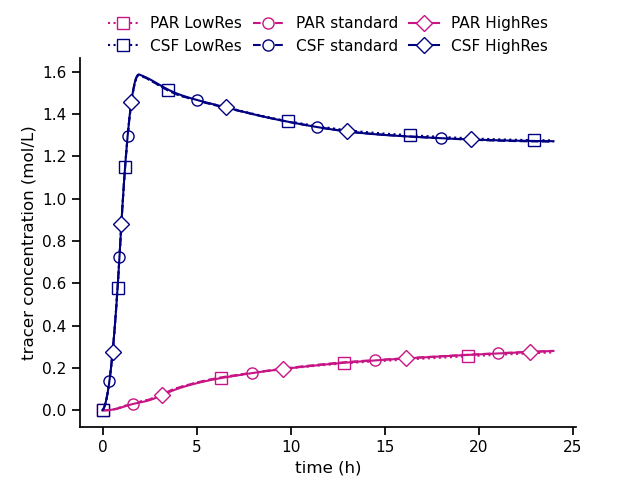
\includegraphics[width = 1 \linewidth]{figures/mesh_refinement_par_csf_mean.png}
        \caption{Mean tracer concentration in CSF and parenchyma under mesh refinement}
    \end{subfigure}
    \begin{subfigure}[b]{0.45\textwidth}
        \centering
     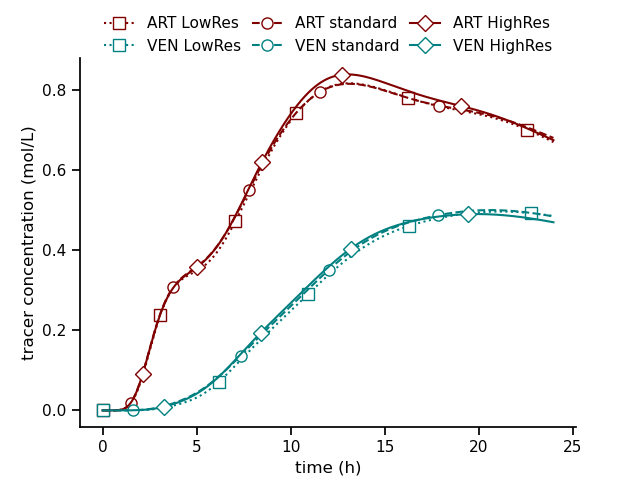
\includegraphics[width= 1 \linewidth]{figures/mesh_refinement_art_ven_mean.png}
         \caption{Mean tracer concentration in PVSs around veins and arteries  under mesh refinement}
    \end{subfigure}
    \caption{Mean tracer concentrations over the first 24\,h after injection on the CSF and parenchyma (a), and the arterial and venous PVS (b) computed on the LowRes, standard and HighRes meshes with a timestep of $dt=120$\,s.}
    \label{fig:mesh_convergence_concentrations}
\end{figure}


\begin{figure}
    \centering
    \begin{subfigure}[b]{0.49\textwidth}
        \centering
        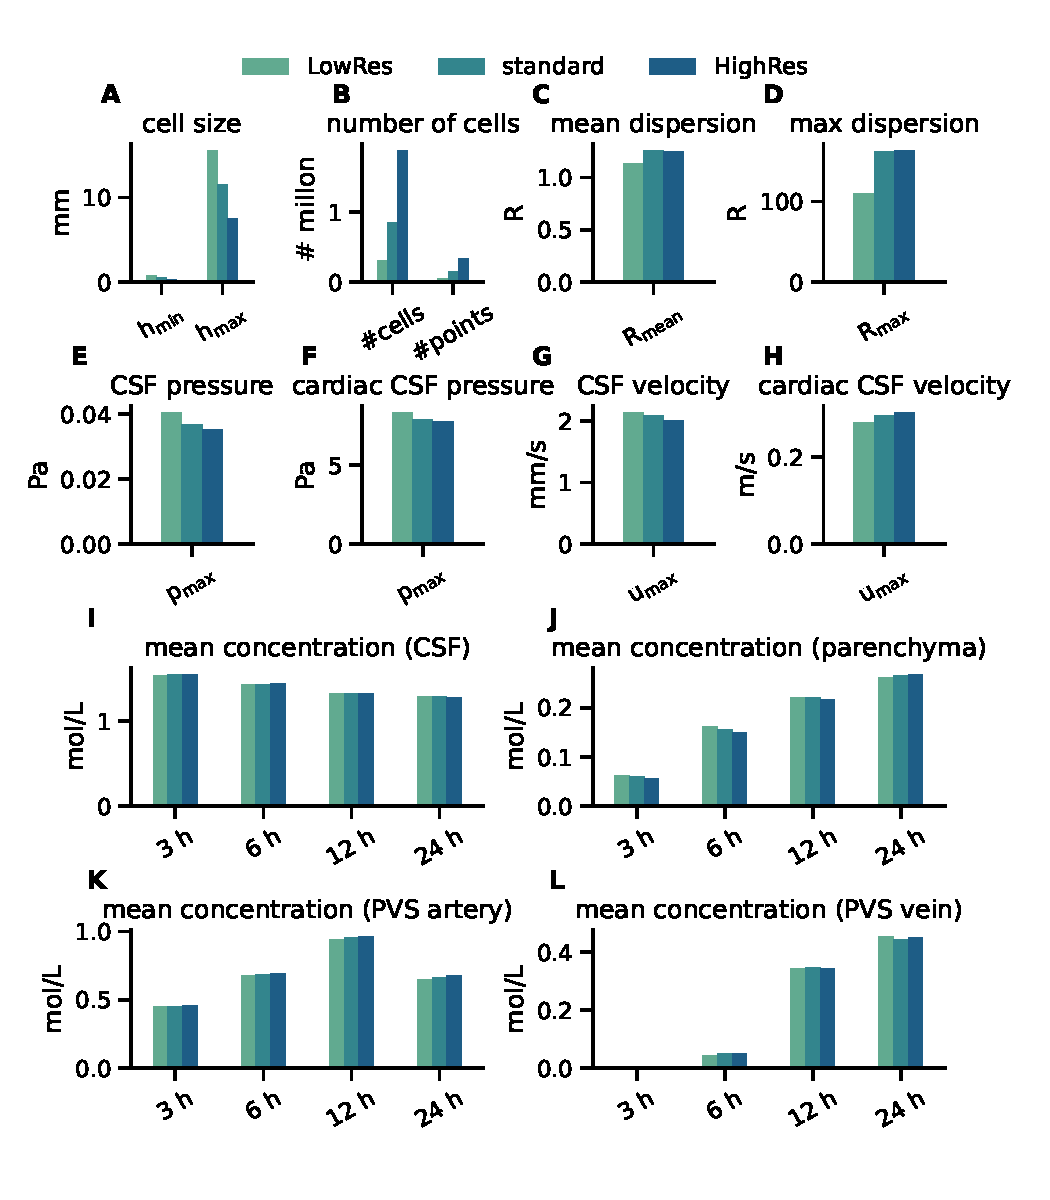
\includegraphics[trim={0.5cm 1cm 0.05cm 0.8cm}, clip, width = 1.05 \linewidth]{figures/mesh_refinement.pdf}
        \caption{Convergence of key quantities of interest with mesh refinement}
        \label{fig:mesh_convergence}
    \end{subfigure}
    \begin{subfigure}[b]{0.49\textwidth}
        \centering
     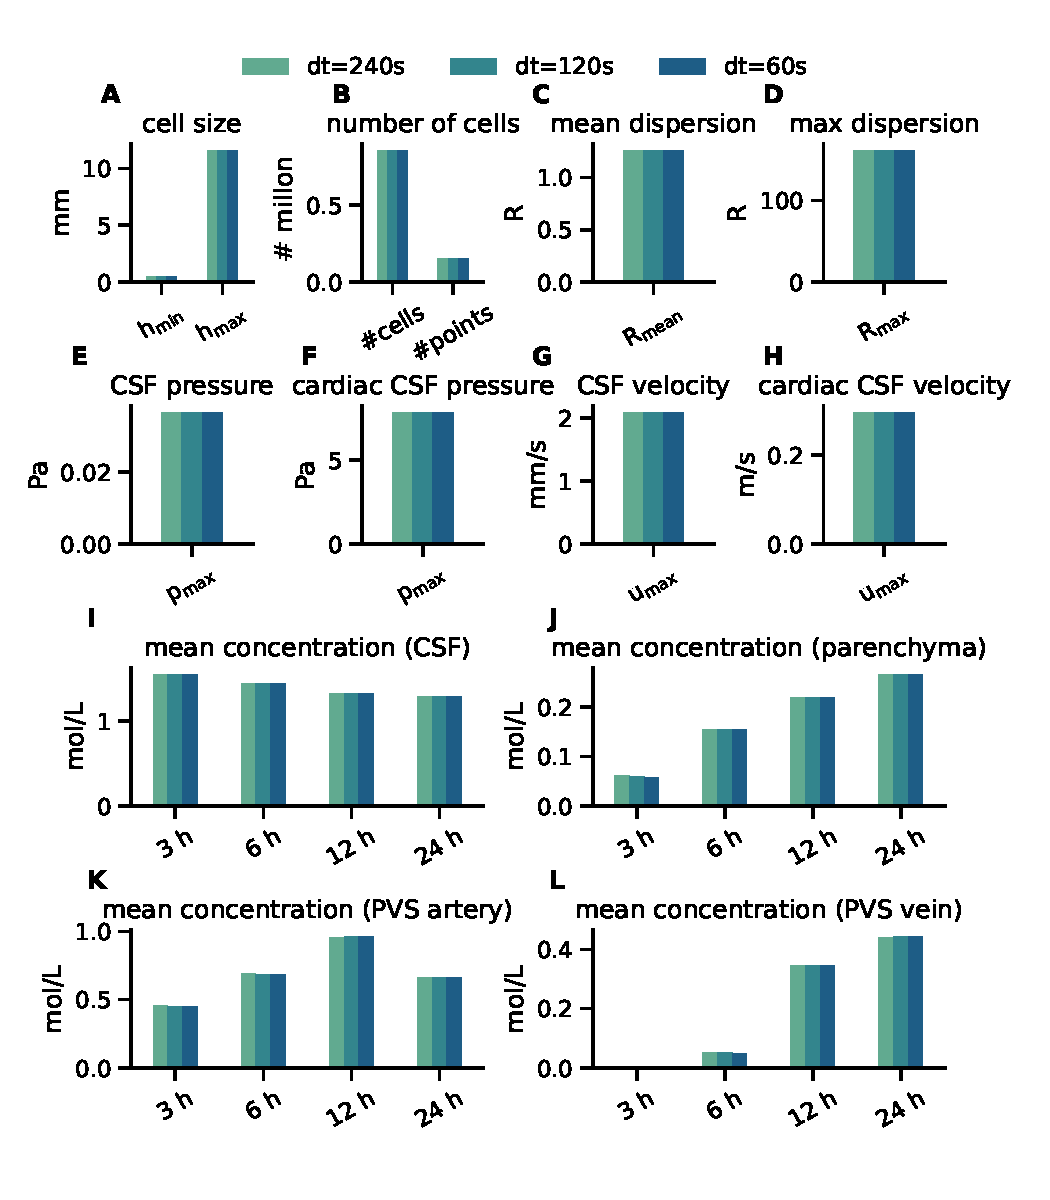
\includegraphics[trim={0.5cm 1cm 0.05cm 0.8cm}, clip,width= 1.05 \linewidth]{figures/time_refinement.pdf}
        \caption{Convergence of key quantities of interest with time refinement}
        \label{fig:time_convergence}
    \end{subfigure}
    \caption{minimal ($\rm h_{min}$) and maximal ($\rm h_{max}$) mesh cell sizes (computed as cell circumradius $\times 2$) (A); number of points and tetrahedral cells in each mesh (B); mean dispersion enhancement factor $R$ (C), maximum dispersion enhancement factor $R$ (D); maximum pressure in steady CSF production flow (E), maximum pressure in cardiac-driven CSF flow (F); maximum CSF velocity in steady CSF production flow (G); maximum CSF velocity in cardiac-driven CSF flow (H);  mean tracer concentration in the CSF, parenchyma, arterial PVS and venous PVS at 3,6,12 and 24\,h (I, J, K and L).}
\end{figure}

\begin{figure}
    \centering
    \begin{subfigure}[b]{0.45\textwidth}
        \centering
        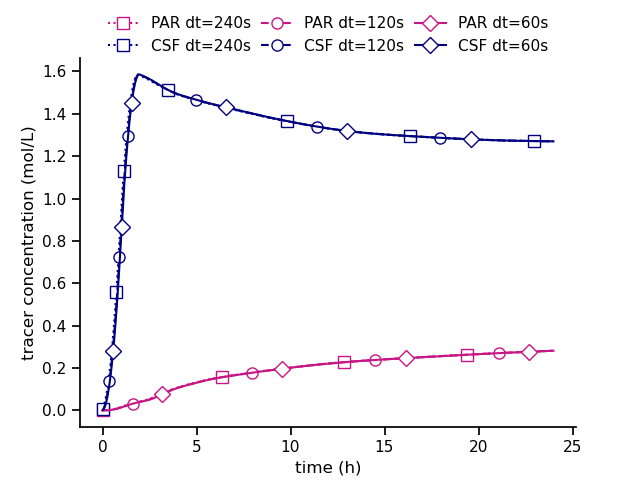
\includegraphics[width = 1 \linewidth]{figures/time_refinement_par_csf_mean.png}
        \caption{Mean tracer concentration in CSF and parenchyma under time step refinement}
    \end{subfigure}
    \begin{subfigure}[b]{0.45\textwidth}
        \centering
     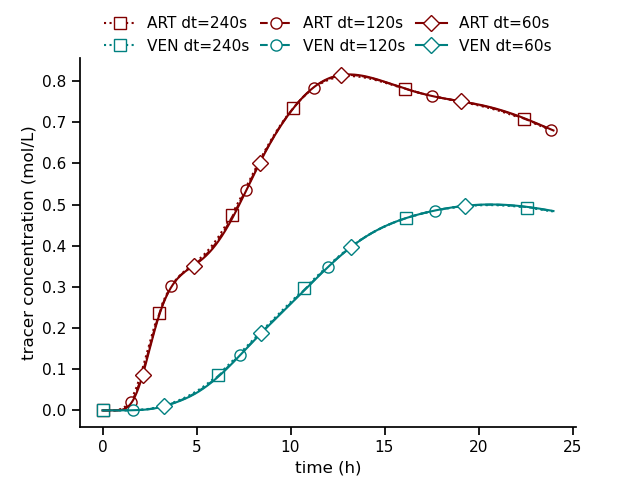
\includegraphics[width= 1\linewidth]{figures/time_refinement_art_ven_mean.png}
         \caption{Mean tracer concentration in PVSs around veins and arteries under time step refinement}
    \end{subfigure}
    \caption{Mean tracer concentrations over the first 24\,h after injection on the CSF and parenchyma (a), and the arterial and venous PVS (b) computed on the standard resolution mesh for timesteps $dt \in \{60, 120, 240 \}$\,s.}    \label{fig:time_convergence_concentrations}
\end{figure}

\newpage
\section{Notes}

Various notes associated with \cite{eide2024functional}:
\begin{itemize}
  \item
    Can observations of tracer indicate compartmentalization without
    the existence of physical barriers but in the presence of
    e.g.~substantial flow? We made observations in this direction in
    \cite{vinje2021brain}, relating to the then-active
    shape-of-perivascular-spaces discussion. We can address this by
    trying to quantify and evaluate the permeability of the PVS-SAS
    interface - comparing model predictions with the timings and
    patterns presented by \cite{eide2024functional}.
  \item
    Do the tracer primarily move from the PVS into the SAS or along
    (more slowly) along the SAS? This is left as an open question by
    \cite{eide2024functional} (page 3)
  \item
    How do altered ICP affect transport? Note that PVSAS transport is
    impaired (delayed) with increasing mean wave amplitude in the ICP
    signal and for iNPH patients (with enlarged PVSAS spaces).
  \item
    Very useful reference for PVS sizes (10--20 mm$^2$ in reference
    patients, 15-70 mm$^2$ in iNPH), and average propagation speeds.
\end{itemize}

\end{document}
